\documentclass[twoside,12pt]{report}
\usepackage[T1]{fontenc}
\usepackage[utf8]{inputenc}
\usepackage{amsmath,amssymb,amsfonts}
\usepackage{amsthm}
\usepackage[polish]{babel}
\usepackage{graphicx}
\usepackage{pdfpages}
\usepackage{hyphenat}
\usepackage{txfonts}
\usepackage{caption}
\usepackage[unicode]{hyperref}
\usepackage{float}
\usepackage{listings}
\usepackage{fancyhdr}
\usepackage{indentfirst}
\usepackage{geometry}
\usepackage{verbatim}
\usepackage{parskip}

\widowpenalty=10000
\clubpenalty=10000
\brokenpenalty 10000 
\sloppy


\geometry{a4paper,left=35mm,right=25mm,top=25mm,bottom=25mm}

\renewcommand{\headrulewidth}{0.1pt}
\renewcommand{\chaptername}{Rozdział}
\renewcommand{\contentsname}{Spis treści}
\renewcommand{\figurename}{Rys.}
\renewcommand{\tablename}{Tab.}
\renewcommand{\lstlistingname}{Listing}
\renewcommand{\listfigurename}{Spis rysunków}
\renewcommand{\listtablename}{Spis tabel}
\renewcommand{\lstlistlistingname}{Spis listingów}
\renewcommand{\bibname}{Bibliografia}

\linespread{1.3} % Jeśli chcesz używać interlinii równej 1,5 jako wartość należy wstawić "1.3".

\pagestyle{fancy}
\fancyhf{}
\fancyhead[LE,RO]{\rightmark}
\fancyfoot[LE,RO]{\thepage}
\setlength{\headheight}{15.13202pt}
\setlength{\parindent}{1.5em}
\setlength{\emergencystretch}{3em}
\urlstyle{rm}

\let\oldsection\chapter
\def\chapter{\cleardoublepage\oldsection}

\newtheorem{definition}{Definicja} % przykład nowego środowiska 
\newtheorem{example}{Przykład}[chapter] % przykład nowego środowiska 
\newtheorem{corollary}{Wniosek}[chapter] % przykład nowego środowiska 

\begin{document}


\includepdf[pages={1,2}]{titlepage.pdf}

\tableofcontents	% generuje spis treści ze stronami !!!

\chapter{Wstęp.} \label{rozdz.wstep} 

\section{Problematyka i~zakres pracy.}

Niniejsza praca obejmuje zagadnienia z~zakresu inżynierii oprogramowania i~sztucznej inteligencji. Głównym jej celem jest stworzenie aplikacji optymalizującej strukturę sieci drogowej.

Problemy komunikacji w~dzisiejszych miastach są wszystkim znane. Zatory drogowe i~korki w~godzinach szczytu są chlebem powszednim. Pomimo wielu prób i~sposobów, wciąż nie istnieje metoda jednoznacznie rozwiązująca tę kwestię. Bezspornie, dotyczy to wszystkich miast na świecie. Z~teoretycznego punktu widzenia, jedynym rozwiązaniem jest komunikacja publiczna. Oczywistym jest jednak, że nigdy nie doprowadzimy do sytuacji, gdy wszyscy mieszkańcy zrezygnują ze swoich pojazdów. Dodatkowo, wiele osób i~usług wymaga oddzielnej formy transportu. W~obliczu tych faktów miasta decydują się na rozwój swojej infrastruktury drogowej. Budowa nowych tras oraz poszerzanie starych przynosi nadzieję mniejszych zatorów a~co za tym idzie, szybszego przejazdu do celu. Niestety, historia pokazuje, że takie inwestycje nie zawsze przynoszą oczekiwane korzyści.

Teorii próbujących wytłumaczyć te zjawiska, jak również dowodów, które je popierają lub obalają jest wiele. Jedną z~najpopularniejszych oraz taką która została wykorzystana w~niektórych miastach na świecie jest paradoks Braessa\cite{braess}. Jest to twierdzenie matematyczne orzekające, że w~pewnym modelu ruchu drogowego czasy podróży pojazdów mogą ulec wydłużeniu po dodaniu do sieci drogowej nowego połączenia. Ma ono również  zastosowanie w~przypadku  sieci komputerowych oraz istnieją jego analogie dla doświadczeń fizycznych.

Moim celem jest opracowanie metody, która dla danej struktury sieci drogowej zmodyfikuje ją wykorzystując prawidłowość z~powyższego paradoksu. W~efekcie poprzez zamknięcie wybranych ulic w~danej sieci drogowej, średni czas podróży powinien ulec skróceniu.

\section{Metoda badawcza i~cel pracy.}
\subsubsection{Studia literaturowe.}
Moje badania rozpocząłem od poszukiwania źródeł traktujących o~opisywanym przeze mnie problemie. Paradoks Braessa został sformułowany w~1970 roku i~był od tego czasu wykorzystywany przy planowaniu przestrzeni i~infrastruktury wielu miast, np:

\begin{itemize}
\item Korea, Seul, likwidacja m.in. estakad Cheonggyecheon,
\item Niemcy, Stuttgart, likwidacja dróg zbudowanych w~latach 60,
\item USA, Nowy Jork, czasowe zamknięcie ulicy 42,
\item USA, Winnipeg.\cite{urban}
\end{itemize}  

\subsubsection{Propozycja rozwiązania problemu.}
Oczywistym rozwiązaniem problemu komunikacji mogłoby być stworzenie idealnej sieci odpowiadającej potrzebom danego miasta. Rozbudowa lub modyfikacja tej infrastruktury jest jednak kosztowna i~czasochłonna. Dlatego zdecydowałem się na przetestowanie rozwiązania zaproponowanego przez Braessa. Ponieważ istnieją prace negujące lub podważające paradoks\cite{newinsights} , zdecydowałem by przy potwierdzaniu wyniku optymalizacji nie kierować się wyłącznie założeniami zawartymi w~twierdzeniu.

\subsubsection{Opis zastosowania algorytmów genetycznych.}
Ponieważ nie znalazłem żadnych przesłanek wykazujących jednoznaczną ocenę co do słuszności zamknięcia danej ulicy, zdecydowałem się losowe przeszukiwanie przestrzeni rozwiązań.~Jednym z~rozwiązań w~przypadku takich poszukiwań są algorytmy genetyczne, na które się zdecydowałem w~swojej pracy.

\subsubsection{Przedstawienie oceny optymalizacji.}
Paradoks Braessa zakłada dość oczywiste potwierdzenie swojej wiarygodności. Zdecydowałem się więc na zastosowanie zewnętrznego systemu oceny. Taką rolę spełniają systemy symulacji. System, który wybrałem działa zupełnie oddzielnie od metody twierdzenia, symulując rzeczywisty ruch na danej sieci drogowej. Wynik symulacji jest jednoznaczną wartością liczbową, przedstawiającą średni czas przejazdów wszystkich agentów biorących udział w~danym scenariuszu. Zakładając stały zestaw agentów dla zmieniających się w~wyżej opisany sposób sieci, dążymy oczywiście do minimalizacji średniego czasu przejazdu.

\subsubsection{Ocena możliwości wdrożenia proponowanych rozwiązań.}
Paradoks Braessa nie jest jedynym twierdzeniem traktującym o~problemach komunikacyjnych miast. Wiele teorii jest opartych głownie na socjologicznych lub psychologicznych założeniach\footnote{np. paradoks Downsa Thomsona\cite{downs} czy prawo Lewisa Mogridge’a\cite{lewis}}. Są jednak niemniej ważne.
Biorąc pod uwagę złożoność problemu, wynik otrzymany podczas eksperymentu nie może być dowodem ani decydującym głosem w~decyzjach dotyczących ustalaniu rzeczywistego ruchu drogowego miasta. 


\section{Przegląd literatury w~dziedzinie.}
By przybliżyć temat problemów komunikacyjnych i~rozwiązania zaproponowanego przez Braessa polecam pracę magisterską \textit{Leslie Arthura Keith Bloy}\cite{investigation}. W~pracy zostały opisane także inne (wymieniane również przeze mnie) twierdzenia. Publikacja \textit{Reducing the Effects of the Braess Paradox with Information Manipulation}\cite{reducingtheeffects} jest bardzo dobrym uzupełnieniem tematu o~interesującą mnie kwestię symulacji wieloagentowych. Prezentuje ona różnice w~wynikach dla przypadku losowego wyboru drogi przez agentów oraz tej wybranej przy użyciu inteligencji kolektywnej\footnote{ang. Collective Intelligence (COIN)}. 

Zbiorowa praca napisana na potrzeby międzynarodowej konferencji dotyczącej technologii symulacji\cite{reducingtheeffects} jest pozycją, która opisuje podobny do podejmowanego przeze mnie problem. Mianowicie skupia się na modyfikacjach drogi poprzez zmiany dostępności jej składowych.

W zupełnie oddzielnej tematyce, algorytmów genetycznych, polecę bardzo łatwo dostępną pozycję, która jest wstępem do tematu\cite{gene}. Wybrałem ją głównie ze względu na prosty opis problemu oraz brak zaawansowanych przykładów, które tylko skomplikowałyby dla mnie ujęcie prostego problemu.

\section{Układ pracy.}
Tematem pracy jest optymalizacja struktury sieci drogowej, zaś za główny cel przyjęto stworzenie rozwiązania, które wykorzystując algorytmy genetyczne odnajdzie najlepsze rozwiązanie.
 
Rozdział \ref{rozdz.wstep} zawiera wstęp i~cele pracy. W~rozdziale \ref{rozdz.optymalizacja} przybliżam istotę optymalizacji struktur sieci drogowych
oraz opisuję teoretycznie wykorzystane przeze mnie rozwiązania. W~rozdziale \ref{rozdz.technologie} wymieniam technologie, w~których wykonałem aplikację oraz przybliżam zewnętrzne biblioteki, o~które oparłem swoje rozwiązanie. Głównym rozdziałem pracy jest rozdział \ref{rozdz.opis},
w którym przedstawiam wykonaną aplikację oraz wyniki optymalizacji przykładowej sieci. W~rozdziale podsumowującym \ref{rozdz.podsumowanie}, zawarłem wnioski oraz możliwości rozwoju pracy. Po rozdziale 5, podsumowującym, załączam spis rysunków, tabel, listingów i~bibliografie, w~tej kolejności.

\chapter{Optymalizacja struktury sieci drogowej.}\label{rozdz.optymalizacja} 
\section{Podstawowe definicje.}

\begin{definition}\label{Graf nieskierowany}
\textbf{Grafem (nieskierowanym)} nazywamy parę zbiorów $(V,E)$. Elementy zbioru $V$ nazywają się \textit{wierzchołkami}, natomiast elementy zbioru $E$ nazywają się \textit{krawędziami}. Każda krawędź jest parą wierzchołków, tzn. $E \subseteq {{u,v}:u,v \in V}$\cite{grafy}.
\end{definition}

\begin{figure}[ht]
\begin{center}
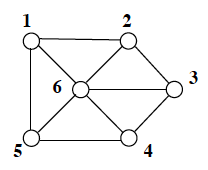
\includegraphics[width=0.40\textwidth]{img/graf1}
\caption{Przykładowy graf nieskierowany.} 
\end{center}
\end{figure}

Przykładowy graf nieskierowany może zostać opisany przez zbiory:
\begin{center}
\begin{math}
V=\{1,2,3,4,5,6\} \hspace*{40px} E=\{\{1,2\},\{2,3\},\{3,4\},\{4,5\},\{6,5\},\{6,1\},\{2,6\},\{3,6\},\{4,6\}\}
\end{math}
\end{center}

\vspace*{30px}
\begin{definition}\label{Graf skierowany}
\textbf{Grafem skierowanym} nazywamy taki graf, w~którym każda krawędź ma zdefiniowany początek i~koniec, tzn. żeby pary były uporządkowane. Wtedy $E \subseteq V \times V = {{u,v}:u,v \in V}$.
Krawędź $(u,v)$ najłatwiej wyobrazić sobie jako strzałkę od $u$ do $v$, dlatego często będziemy oznaczać ją przez $u \rightarrow v$\cite{grafy}.
\end{definition}

\begin{figure}[ht]
\begin{center}
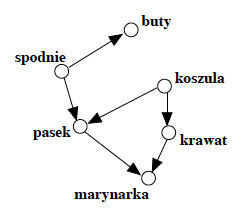
\includegraphics[width=0.40\textwidth]{img/graf2}
\caption{Przykładowy graf skierowany.} 
\end{center}
\end{figure}

Przykładowy graf skierowany może zostać opisany przez zbiory:
\newline
\begin{math}
V=\{spodnie, buty, pasek, koszula, krawat, marynarka\}
\end{math}
\newline
\begin{math}
E=\{\{spodnie \rightarrow buty\},\{spodnie  \rightarrow pasek\},
	\{pasek \rightarrow koszula\},\{koszula \rightarrow krawat\},
	\{pasek \rightarrow marynarka\},\{krawat \rightarrow marynarka\}\}
\end{math}

\section{Sieć drogowa w~postaci grafu}
W przypadku sieci drogowej mamy oczywiście do czynienia z~abstrakcyjną strukturą sieci. Przez sieć drogową rozumiemy bowiem układ dróg lub ulic np. w~mieście. Podczas swoich badań posługuję się zawsze pewnym fragmentem większej sieci. Najlepiej te dane zobrazuje poniższy przykład.

\begin{figure}[ht]
\begin{center}
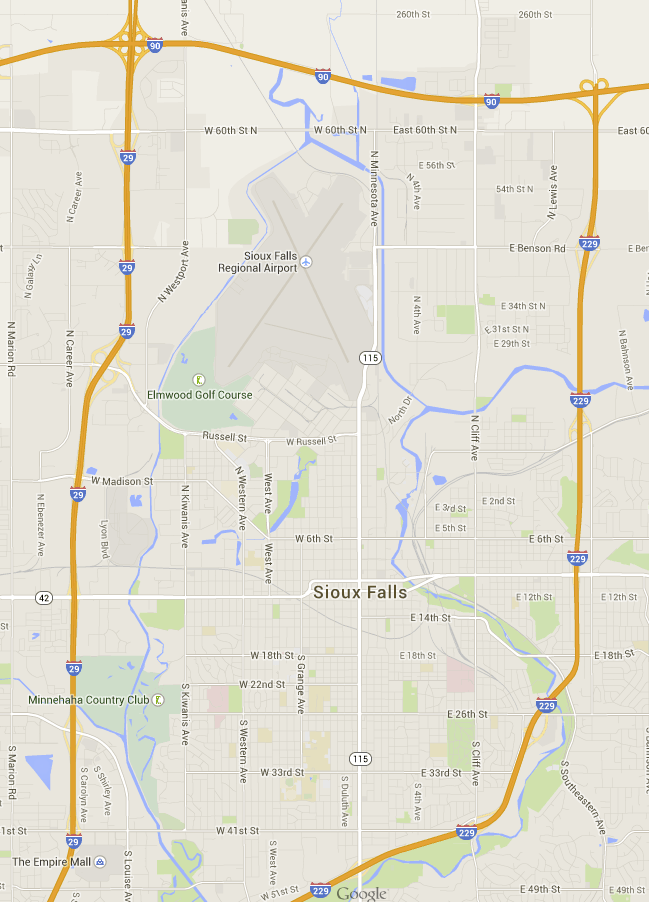
\includegraphics[width=0.35\textwidth]{img/siec}
\caption{Fragment sieci drogowej miasta Sioux Falls, Południowa Dakota.} 
\end{center}
\end{figure}

Posługując się powyższymi definicjami, tworząc graf z~pewnej sieci drogowej, przyjmujemy, że zbiorem $V$, wierzchołków są skrzyżowania, natomiast zbiór krawędzi $E$ odnosi się do ulic pomiędzy tymi skrzyżowaniami.
W mojej pracy posługuję się zawsze grafem skierowanym. W~związku z~tym, w~przypadku ulic dwukierunkowych tworzę parę krawędzi z~odpowiednimi kierunkami, nawet jeśli ulice nie są rozłączne w~rzeczywistości.

W celu potwierdzenia wiarygodności powyższego przykładu prezentuję graf nałożony na mapę miasta\cite{siux}.

\vspace*{30px}
\begin{figure}[h]
\begin{flushleft}
	\begin{minipage}[]{.45\textwidth}
	\centering
	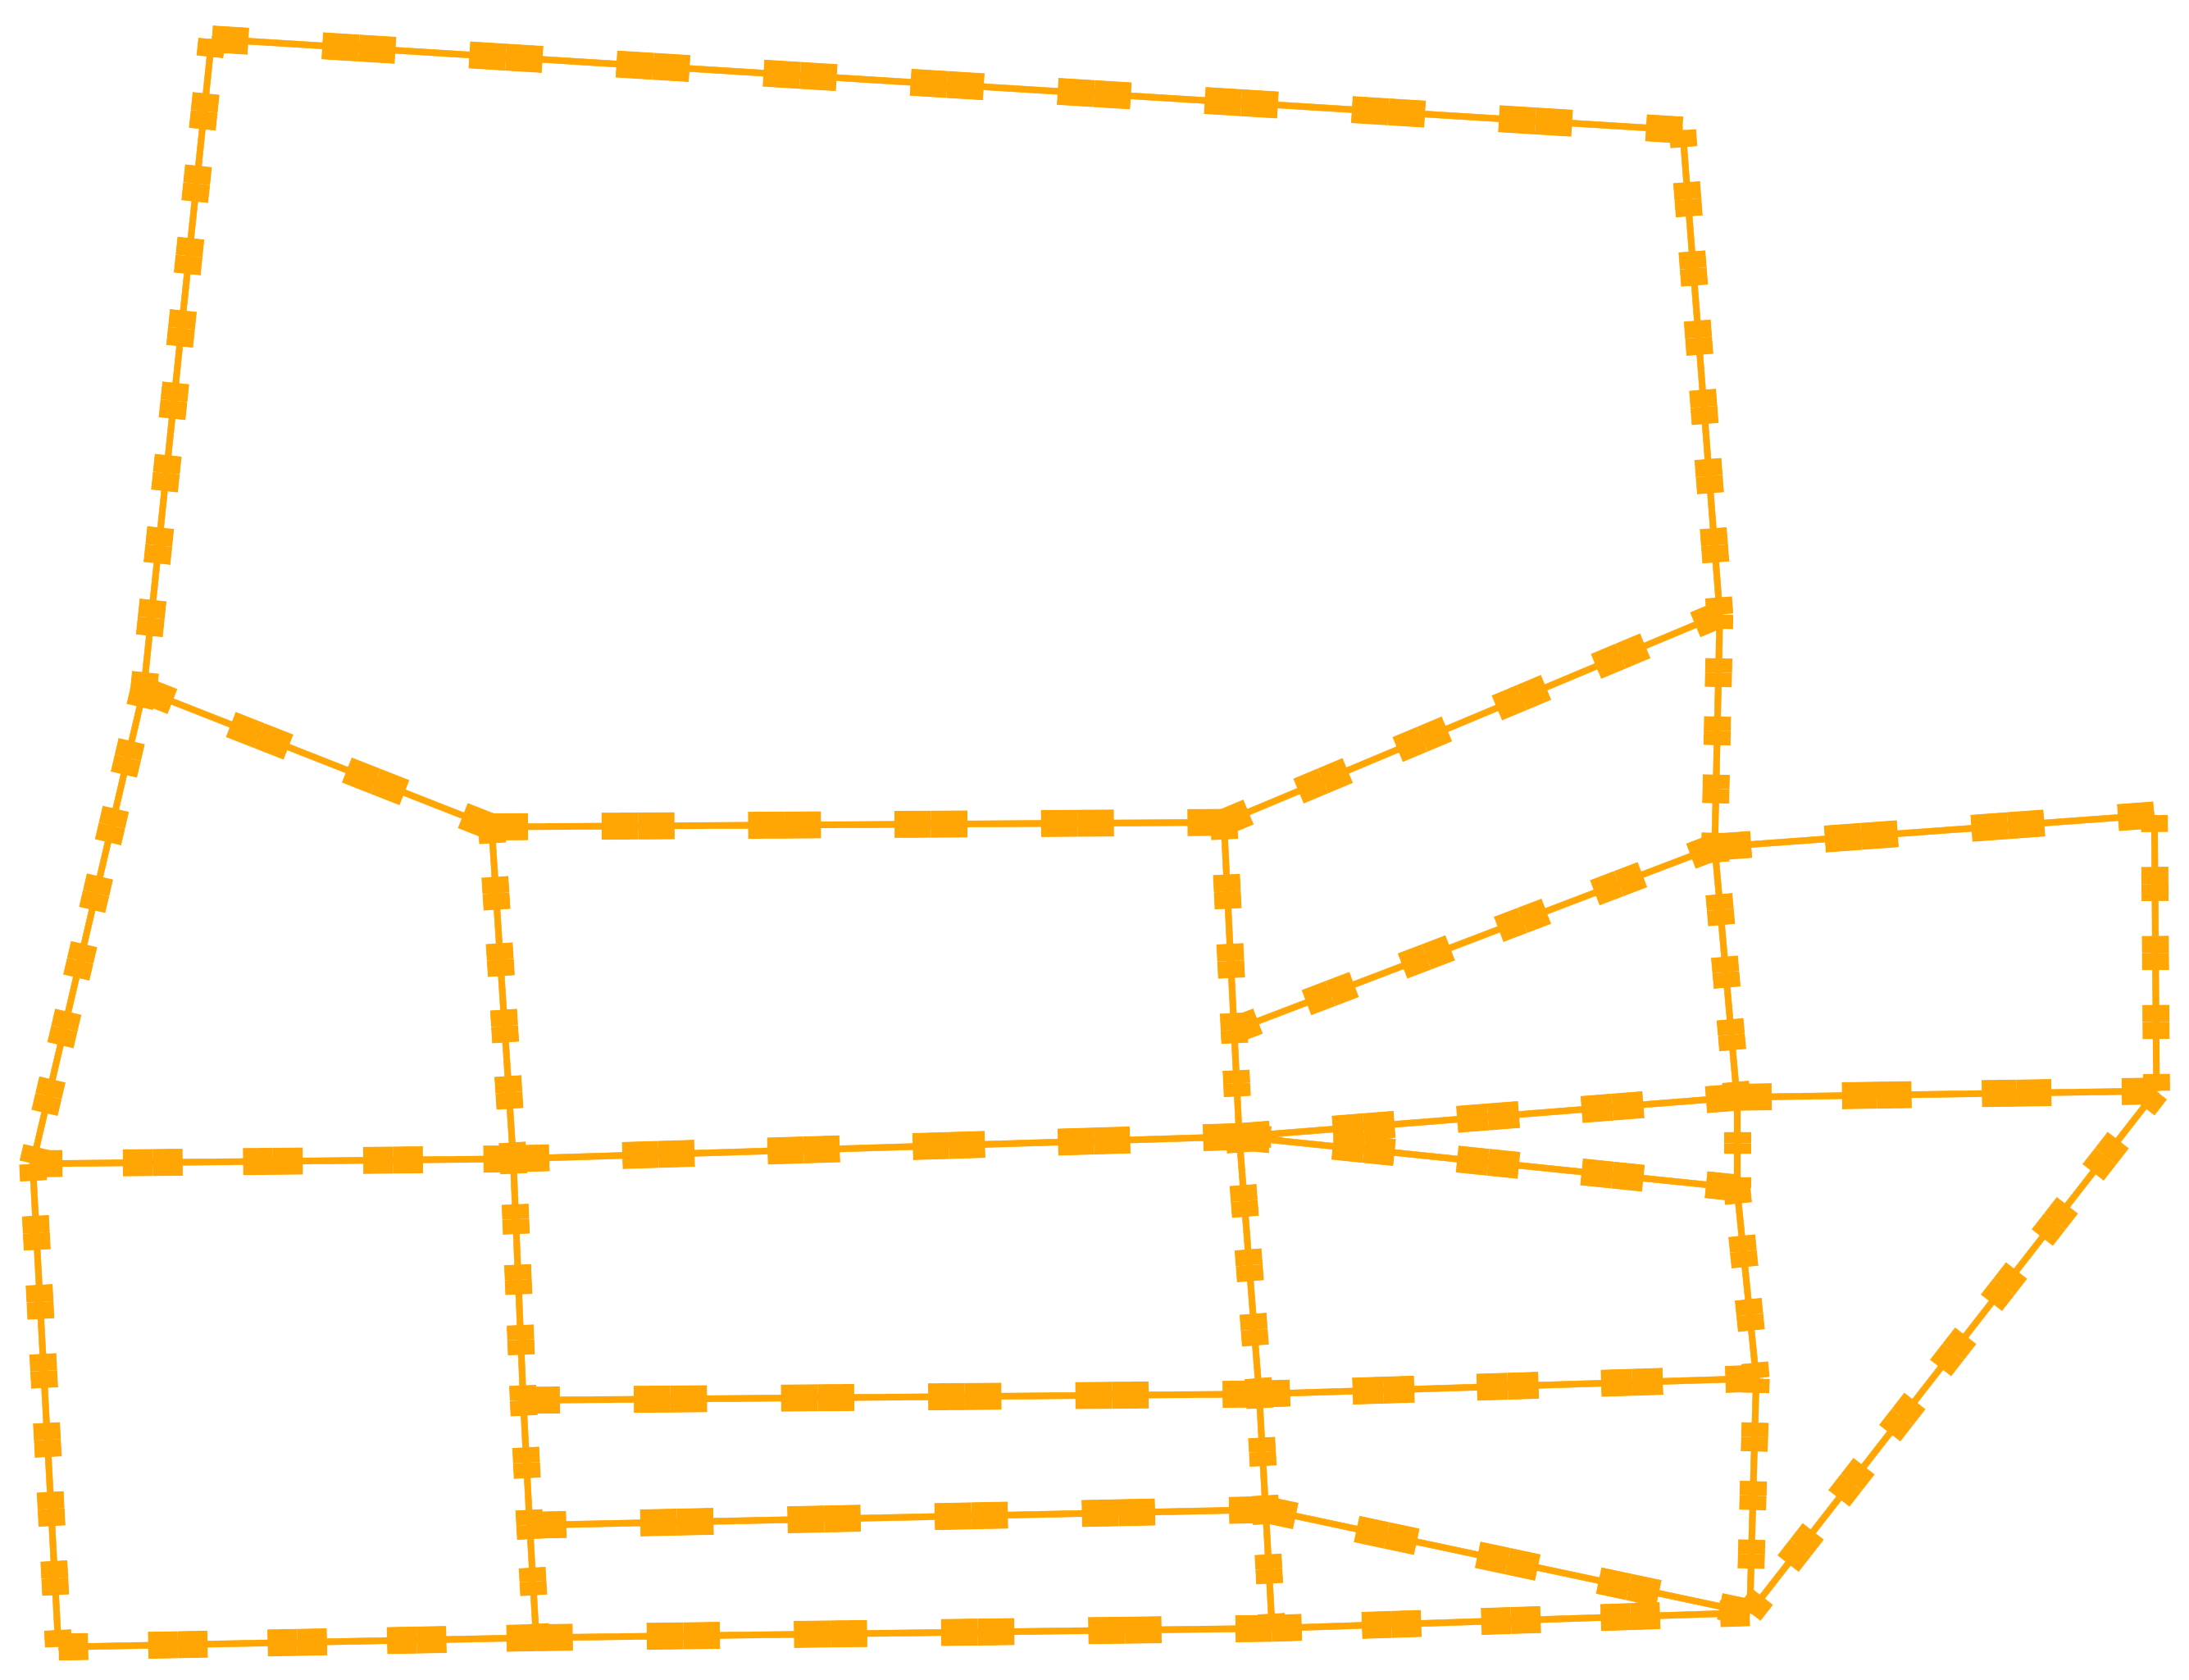
\includegraphics[width=\linewidth]{img/graf}
	\caption{Siec drogowa miasta Sioux Falls w postaci grafu.}
	\end{minipage}%
\end{flushleft}
\begin{flushright}
	\begin{minipage}[]{.45\textwidth}
	\centering
	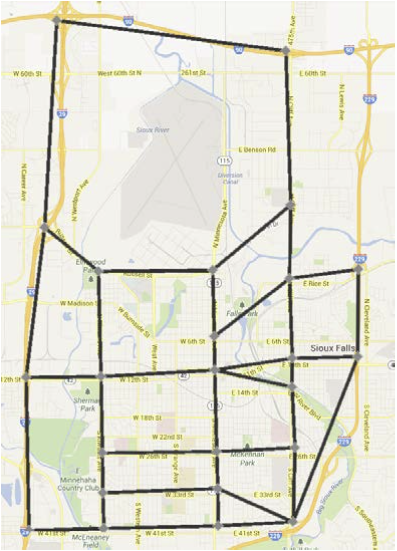
\includegraphics[width=\linewidth]{img/dopasowanie}
	\caption{Graf z dopasowaną geometrią.}
	\end{minipage}
\end{flushright}
\end{figure}

\section{Paradoks Braessa.}

Jak już wcześniej wspomniałem, jest to twierdzenie matematyczne orzekające, że w~pewnym modelu ruchu drogowego czasy podróży pojazdów mogą ulec wydłużeniu po dodaniu do sieci drogowej nowego połączenia. Autorem twierdzenia jest niemiecki matematyk Dietrich Braess\cite{braess}. Paradoks działa w~oparciu o~model ruchu drogowego, który ma następujące cechy:

\begin{enumerate}
\item Sieć drogowa składa się ze skończenie wielu węzłów i~łączących je odcinków dróg
\item Po sieci porusza się skończenie wiele pojazdów, każdy z~nich ma wyznaczony węzeł startowy i~węzeł docelowy
\item Odcinki dróg mają przypisane sobie czasy przejazdu, przy czym czasy te mogą zależeć od liczby pokonujących dany odcinek pojazdów.
\item Układ sieci drogowej i~czasy przejazdu poszczególnych odcinków są znane pojazdom
\item Celem pojazdów jest przejazd przez sieć z~węzłów początkowych do docelowych po trasie złożonej z~odcinków drogowych tak, by zminimalizować łączny czas ich pokonania
\item Decyzje o~wyborze tras pojazdy podejmują indywidualnie i~niezależnie od siebie
\end{enumerate}
Przedstawię paradoks w~oparciu o~przykład z~oryginalnego artykułu Dietricha Braessa\cite{paradox}.

\subsection{Przykładowy, wyjściowy układ drogowy.}
\subsubsection{Sieć drogowa i~auta}

Przykład sytuacji, w~której ujawnia się paradoks Braessa jest skonstruowany z~czterech miast $A$, $B$, $X$ i~$Y$. Są one połączone odcinkami drogowymi jak na rysunku i~z~następującymi czasami przejazdu, przy czym $p$ oznacza gęstość ruchu w~tysiącach aut.

\vspace*{15px}
\begin{figure}[h]
\begin{flushleft}
\begin{minipage}{.50\textwidth}
Autostrady:\newline
AX, $t_{AX}(p) =  50 + p$ min\newline
YB, $t_{YB}(p) =  50 + p$ min\newline

\vspace*{15px}
Drogi lokalne:\newline
AY, $t_{AY}(p) =  10p$ min\newline
XB, $t_{XB}(p) =  10p$ min\newline

\vspace*{15px}
Aut jest 6000 i wszystkie mają za zadanie przejechać trasę z $A$ do $B$.
\end{minipage}%
\end{flushleft}
\begin{flushright}
	\begin{minipage}{.50\textwidth}
	\centering
	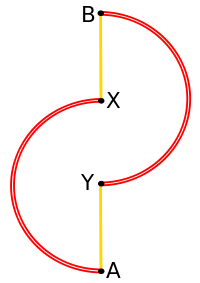
\includegraphics[width=0.7\textwidth]{img/braess1}
	\caption{Wyjściowy układ drogowy}
	\end{minipage}
\end{flushright}
\end{figure}


\subsubsection{Analiza równowagi Nasha}

Każde auto musi zdecydować się na wybór trasy albo $AXB$ albo $AYB$.

Równowaga Nasha to taka sytuacja, w~której każdy z~samochodów spowoduje wydłużenie swojego czasu jazdy, zmieniając decyzję co do wyboru trasy przy niezmienionych decyzjach pozostałych aut.
\newline\newline
Jeśli $p$ i~$q$ to liczby aut w~tysiącach pokonujących odpowiednio trasy $AXB$ i~$AYB$, otrzymujmy równania:

\begin{center}
\begin{math}
p+q = 6 \newline
t_{AX}(p)+t_{XB}(p) = t_{AY}(q) + t_{YB}(q) \newline
50+p+10p = 10q+50+q \newline
\end{math}
\end{center}
rozwiązaniem jest $p=q=3$.
Przy tej gęstości ruchu pokonanie obu dostępnych tras zabiera $50+3+30=83$ minuty.

\subsection{Przykładowy, uzupełniony układ drogowy.}
\subsubsection{Sieć drogowa i~auta}
Do wyjściowego układu drogowego dodana zostaje autostrada:

\vspace*{60px}
\begin{figure}[h]
\begin{flushleft}
	\begin{minipage}{.50\textwidth}
	Autostrady:\newline
	YX, $t_{YX}(p) =  10 + p$ min\newline
	
	\vspace*{15px}
	Aut jest nadal 6000 i wszystkie mają za zadanie przejechać trasę z $A$ do $B$.
	\end{minipage}%
\end{flushleft}
\begin{flushright}
	\begin{minipage}{.50\textwidth}
	\centering
	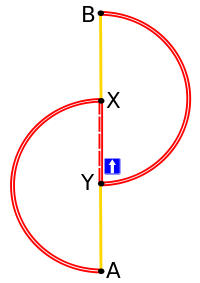
\includegraphics[width=0.7\textwidth]{img/braess2}
	\caption{Uzupełniony układ drogowy}
	\end{minipage}
\end{flushright}
\end{figure}

\subsubsection{Analiza równowagi Nasha}

Jeśli $p$, $q$ i~$r$ to liczby aut w~tysiącach pokonujących odpowiednio trasy $AXB$, $AYB$ i~$AYXB$, otrzymujmy równania:

\begin{center}
\begin{math}
p+q+r = 6 \newline
t_{AX}(p)+t_{XB}(p+r) = t_{AY}(q+r) + t_{YB}(q) = t_{AY}(q+r)+t_{YX}(r)+t_{XB}(p+r)\newline
50+p+10(p+r) = 10(q+r)+50+q = 10(q+r)+ 10 + r + 10(p+r)\newline
\end{math}
\end{center}
rozwiązaniem jest $p=q=r=2$.
Czas przejazdu każdej z~tych dróg wynosi wówczas $50+2+10(2+2)=92$ minuty.

\subsection{Wyjaśnienie intuicyjne.}
Wąskim gardłem systemu są drogi lokalne, na których czas przejazdu bardzo szybko wzrasta wraz z~intensywnością ruchu. Po pojawieniu się dodatkowej drogi dostępna staje się nowa trasa, prowadząca oprócz nowego skrótu YX tylko drogami lokalnymi.

Z perspektywy całości systemu nowy odcinek drogowy odciąża ruch na autostradach, gdzie jest to mało odczuwalne, a~w~zamian jeszcze bardziej zagęszcza ruch na drogach lokalnych, powodując wydłużenie czasu podróży.

\section{Graf skierowany silnie spójny.}
Na potrzeby symulatora, sieć drogowa przedstawiona w~postaci grafu skierowanego musi spełniać warunek silnej spójności. 
\newline
\begin{definition}\label{Graf silnie spójny}
\textbf{Grafem skierowanym silnie spójnym} nazywamy graf skierowany w~którym jest możliwe dotarcie do każdego wierzchołka zaczynając z~dowolnego innego poprzez dowolną ilość krawędzi. Wszystkie wierzchołki w~grafie skierowanym silnie spójnym muszą zatem posiadać przynajmniej jedną krawędź wchodzącą i~wychodzącą\cite{silniespojny}.
\end{definition}

W sprawdzaniu grafu pod względem spójności, wykorzystuję algorytm Tarjana do znajdowania składowych silnie spójnych.
\newline
\begin{definition}\label{Algorytm Tarjana}
Podstawowym założeniem \textbf{algorytmu Tarjana} jest przeszukiwanie grafu w~głąb zaczynając od dowolnego wierzchołka wybranego w~sposób arbitralny. Tak jak w~przypadku klasycznego przeszukiwania w~głąb, każdy sąsiadujący wierzchołek po odwiedzeniu zostaje oznaczony i~algorytm nigdy ponownie go nie odwiedza. Dzięki temu, tworzymy kolekcję przeszukanych drzew, która jest drzewem rozpinającym grafu. Składowe silnie spójne są następnie odnajdowane jako poddrzewa, a~korzenie tych poddrzew są nazywane korzeniami składowych silnie spójnych. Każdy wierzchołek grafu może być wybrany na korzeń składowej silnie spójnej jeśli zostanie wybrany jako pierwszy wierzchołek podczas przeszukiwania w~głąb.
\end{definition}

\vspace*{15px}

\begin{definition}
\textbf{Składowa silnie spójna} (ang. strongly connected component) jest maksymalnym pod grafem, w~którym istnieją ścieżki pomiędzy każdymi dwoma wierzchołkami. Jeśli pod graf ten obejmuje wszystkie wierzchołki grafu, to mówimy, że dany graf skierowany jest silnie spójny (ang. strongly connected digraph). W~grafach nieskierowanych każdy graf spójny jest również silnie spójny.
\end{definition}

\begin{figure}[ht]
\centering
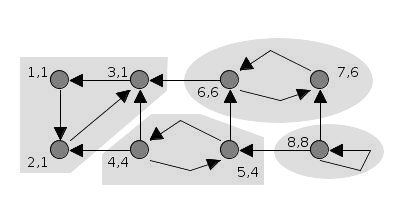
\includegraphics[width=0.6\textwidth]{img/tajran}
\caption{Przykładowy graf z zaznaczonymi składowymi silnie spójnymi.}
\end{figure}

W efekcie, zawsze przed rozpoczęciem symulacji sprawdzam, czy graf jest grafem skierowanym silnie spójnym lub dokładniej mówiąc, czy posiada tylko jedną składową silnie spójną.

\section{Klasyczny algorytm genetyczny.}

Idea algorytmu genetycznego została zaczerpnięta z~nauk przyrodniczych opisujących zjawiska doboru naturalnego i~dziedziczenia. Mechanizmy te polegają na
przetrwaniu osobników najlepiej dostosowanych w~danym środowisku, podczas gdy
osobniki gorzej przystosowane sa eliminowane. Z~kolei te osobniki, które przetrwają
- przekazują informacje genetyczna swoim potomkom. Krzyżowanie informacji genetycznej otrzymanej od ”rodziców” prowadzi do sytuacji, w~której kolejne pokolenia sa przeciętnie coraz lepiej dostosowane do warunków środowiska; mamy wiec tu do czynienia ze swoistym procesem optymalizacji. 

\subsection{Podstawowe pojecia algorytmów genetycznych}

\begin{definition}
\textbf{Populacją} nazywamy zbiór osobników o~określonej liczebności.
\end{definition}

\vspace*{10px}

\begin{definition}
\textbf{Osobnikami} populacji w~algorytmach genetycznych są zakodowane w~postaci chromosomów zbiory parametrów zadania, czyli rozwiązania, określone też jako punkty
przestrzeni poszukiwań.~Osobniki czasami nazywa się organizmami.
\end{definition}

\vspace*{10px}

\begin{definition}
\textbf{Chromosomy} to inaczej łańcuchy lub ciągi kodowe, to uporządkowane ciągi genów.
\end{definition}

\vspace*{10px}

\begin{definition}
\textbf{Gen} – nazywany też cechą, znakiem, detektorem – stanowi pojedynczy element
genotypu, w~szczególności chromosomu. Genotyp, czyli struktura, to zespół chromosomów
danego osobnika. Zatem osobnikami populacji mogą być genotypy albo
pojedyncze chromosomy.
\end{definition}

\vspace*{10px}

\begin{definition}
\textbf{Fenotyp} jest zestawem wartości odpowiadających danemu genotypowi, czyli zdekodowana
struktura, a~wiec zbiorem parametrów zadania (rozwiązaniem, punkt przestrzeni
poszukiwań).
\end{definition}

\vspace*{10px}

\begin{definition}
\textbf{Allel} to wartość danego genu, określona jako wartość cechy lub wariant cechy.
\end{definition}

\vspace*{10px}

\begin{definition}
\textbf{Locus} to pozycja - wskazuje miejsce położenia danego genu w~łańcuchu, czyli chromosomie.
\end{definition}

\vspace*{10px}

\begin{definition}
\textbf{Funkcja przystosowania nazywana tez funkcją dopasowania lub funkcja oceny.} Stanowi ona miarę przystosowania (dopasowania) danego osobnika w~populacji.
\end{definition}

\subsection{Algorytm klasycznego algorytmu genetycznego.}

Na podstawowy (klasyczny) algorytm genetyczny, nazywany także elementarnym
lub prostym algorytmem genetycznym, składają się kroki:

\begin{enumerate}
\item inicjacja czyli wybór początkowej populacji chromosomów,
\item ocena przystosowania chromosomów w~populacji,
\item sprawdzenie warunku zatrzymania,
\item selekcja chromosomów,
\item zastosowanie operatorów genetycznych,
\item utworzenie nowej populacji,
\item wyprowadzenie najlepszego chromosomu.
\end{enumerate}

Najłatwiej wyobrazić sobie powyższe kroki analizując je na schemacie:

\begin{figure}[ht]
\begin{center}
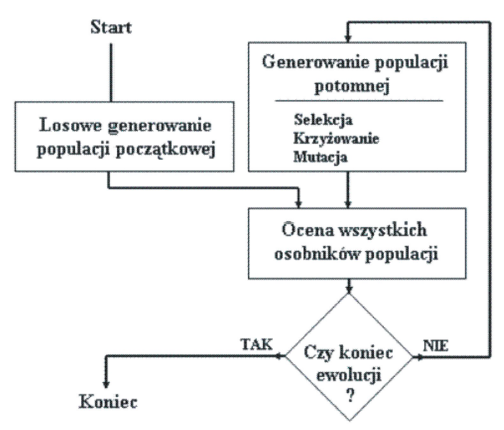
\includegraphics[width=0.6\textwidth]{img/ogolgene}
\caption{Ogólny schemat algorytmu genetycznego.}
\end{center}
\end{figure}

\subsection{Operacje klasyczne, krzyżowanie.}

Operacja krzyżowania jest podstawową operacją algorytmów genetycznych służącą do rekombinacji materiału genetycznego. Operacja opiera się na dwóch chromosomach, których części materiału genetycznego zostają wymieszane w~celu otworzenia nowego chromosomu. Podstawowa operacja krzyżowania opiera się o~jeden punkt krzyżowania i~została przedstawiona na poglądowym schemacie poniżej\cite{gene mutikrzyz}.

\begin{figure}[ht]
\begin{center}
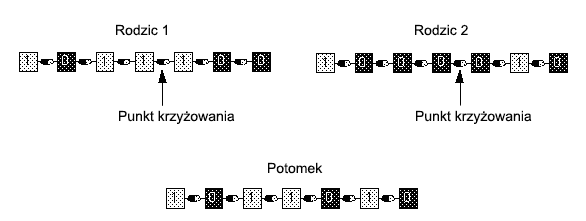
\includegraphics[width=\textwidth]{img/crossover}
\caption{Ogólny schemat operacji krzyżowania.}
\end{center}
\end{figure}

\subsection{Operacje klasyczne, mutacja.}

Proces rekombinacji przez krzyżowanie nie byłby w~stanie odkryć całej przestrzeni poszukiwań, jeżeli dana kombinacja nie byłaby obecna w~sekcjach populacji. To mogłoby prowadzić do błędnego wyniku. Operacja mutacji pozwala na wprowadzenie nowych struktur genetycznych w~obecnej populacji. Dokonuje tego poprzez losową zmianę dowolnego genu w~chromosomie\cite{gene mutikrzyz}.

\begin{figure}[ht]
\begin{center}
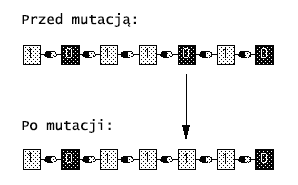
\includegraphics[width=0.55\textwidth]{img/mutation}
\caption{Ogólny schemat operacji mutacji.}
\end{center}
\end{figure}

\section{Użycie grafów w~algorytmie genetycznym.}

W swojej pracy posługuję się przede wszystkim grafami. W~tym wypadku klasyczna odmiana algorytmu genetycznego musiałaby zostać zmodyfikowana na potrzeby wykorzystania grafów jako chromosomów. Dodatkowo wymagałoby to zastosowania nowych sposobów krzyżowania i~mutacji jednostek. 

Zdecydowałem, że zamiast przystosowywać algorytm genetyczny do nowej struktury, przystosuję strukturę do algorytmu. Ponieważ moim zadaniem jest zdecydowanie o~zamknięciu lub nie, danej ulicy (krawędzi grafu) postanowiłem opisać tę strukturę jako listę opisującą ten stan. Zgodnie z~tą myślą, sieć drogowa (graf) jest tłumaczona na tablicę elementów przyjmujących wartości:

\begin{itemize}
\item 1 (prawda) - dla ulicy (węzła), który jest przejezdny,
\item 0 (fałsz) - dla ulicy (węzła) zamkniętego dla ruchu.
\end{itemize}

Tablica tworzona w~ten sposób może być modyfikowana przez algorytm genetyczny, jak również bez problemu mogę z~niej odtworzyć stan obecny sieci drogowej. Za przykład podaję sytuację przedstawioną niżej.


\begin{figure}[ht]
\begin{flushleft}
	\begin{minipage}[c]{.47\textwidth}
	\vspace*{80px}
	\centering
	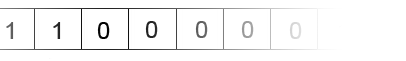
\includegraphics[width=\textwidth]{img/bool}
	\caption{Fragment sieci w postaci tablicy binarnej }
	\label{left-example}
	\end{minipage}%
\end{flushleft}
\begin{flushright}
	\begin{minipage}[c]{.47\textwidth}
	\centering
	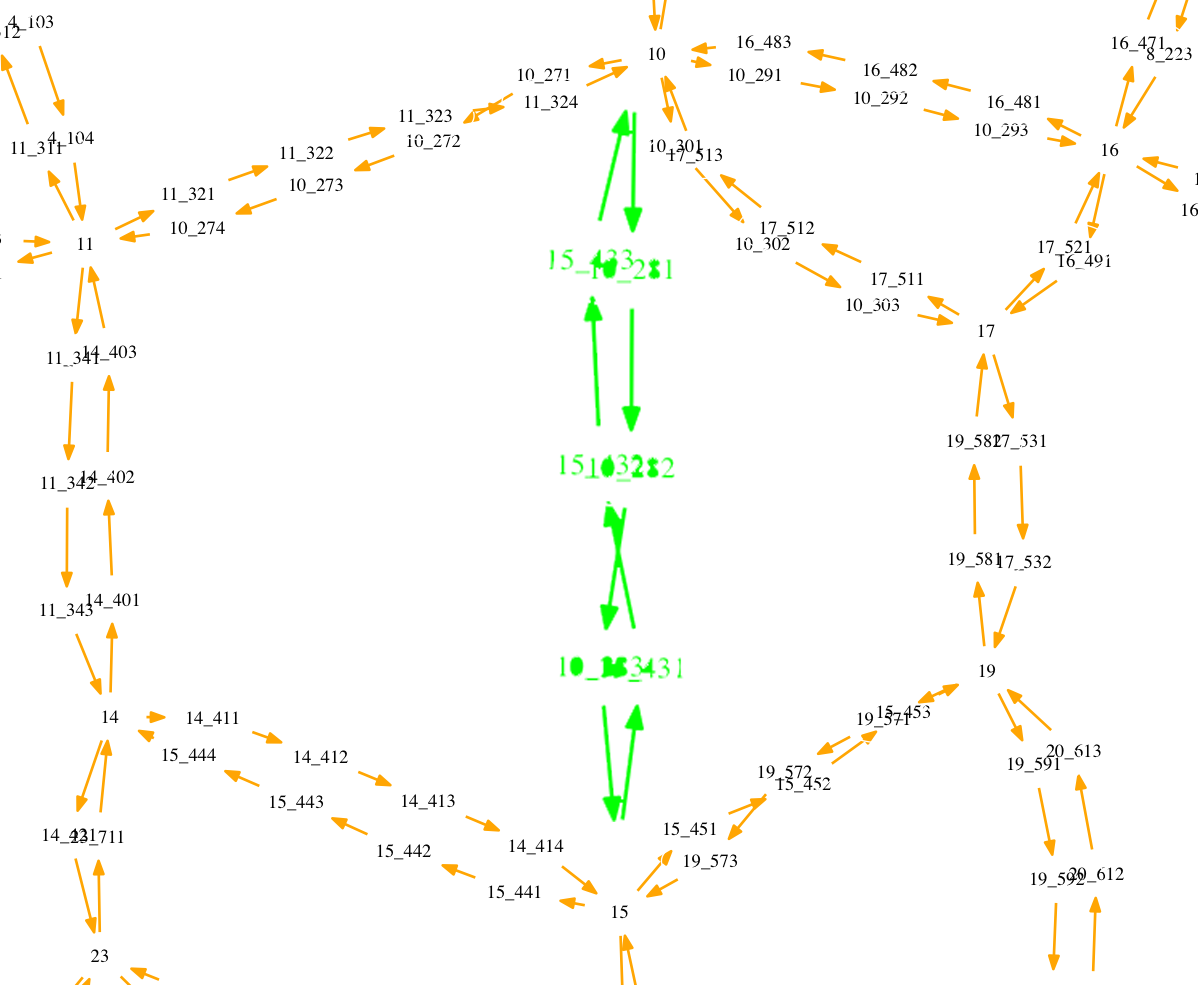
\includegraphics[width=\textwidth]{img/bool-efect}
	\caption{Fragment sieci w postaci grafu}
	\label{right-example}
	\end{minipage}
\end{flushright}
\end{figure}

Przedstawiony na rysunku \ref{left example} fragment sieci zawiera kolejne elementy zerowe, które w~tłumaczeniu na przykładowy graf \ref{right example}, są zaznaczone kolorem zielonym. W~tym przypadku krawędzie te zostaną wyłączone z~ruchu. 

\section{Punkty artykulacji grafu.}

Punktem artykulacji\footnote{ang. articulation point lub cut vertex} jest wierzchołek, którego usunięcie z~grafu spowoduje zwiększenie liczby spójnych składowych. Na rysunku, punktem artykulacji jest wierzchołek$nr 0$.

\begin{figure}[h]
\begin{center}
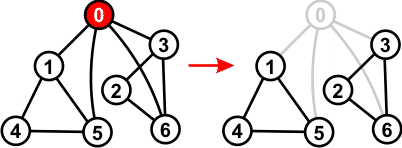
\includegraphics[width=0.7\textwidth]{img/articulation}
\caption{Przykład grafu z zaznaczonym punktem artykulacji.}
\end{center}
\end{figure}

Algorytm poszukiwania punktów artykulacji wykorzystuje przeszukiwanie grafu w~głąb. Podczas nierekurencyjnego przejścia, sprawdza najwyższy poziom zagłębienia, do którego wierzchołki sięgają w~drzewie. Wierzchołek $n$ jest punktem artykulacyjnym wtedy, i~tylko wtedy, jeżeli istnieje poddrzewo z~korzeniem w~punkcie $n$, takie, w~którym żaden poprzednik i~następnik $n$ nie są połączeni w~drzewie DFS. 

Punkty te wykorzystuję, by podczas losowych mutacji i~krzyżowań w~algorytmie genetycznym nie doszło do stworzenia grafu innego niż grafu skierowanego silnie spójnego. Krok sprawdzenia jest wykonywany podczas każdorazowego zamykania drogi, zatem za każdym razem gdy zostaje wprowadzona nowa wartość $"0"$ w~tablicy.

\chapter{Technologie i~metody użyte.}\label{rozdz.technologie} 
\section{Symulator transportu.}

MATSim dostarcza framework\footnote{pl. szkielet do budowy aplikacji} do implementacji szerokiej skali symulacji transportu opartych na agentach. Składa się z~wielu modułów, które mogą zostać połączone lub używane oddzielnie. Moduły można zastępować własnymi implementacjami w~celu przetestowania pojedynczych aspektów pracy\cite{matsim}.

\begin{figure}[ht]
\centering

\includegraphics[width=0.40\textwidth]{img/matsim}
\caption{Logo symulatora transportu MATSim} 
\end{figure}

Oczywiście MATSim nie jest jedynym dostępnym symulatorem transportu. Podobnych rozwiązań jest wiele. Swój wybór jednak motywowałem przede wszystkim dostępnością materiałów szkoleniowych i~przykładowymi scenariuszami. MATSim jest żywym projektem oparty o~licencję open source\footnote{pol. otwarte oprogramowanie}. Dysponuje szerokim zasobem przykładów i~gotowych scenariuszy, w~dodatku udostępniając prace wielu osób na swoim repozytorium.

\section{Algorytmy genetyczne.}

Projekt The Apache Commons jest tworzony przez Apache Software Foundation, formalnie przez Jakarta Project. Głównym celem projektu jest stworzenie wolnego oprogramowania do wielokrotnego użytku w~języku Java. Projekt podzielony jest na trzy główne części: proper, sandbox, i~dormant\cite{math}.

W przypadku głównej części Apache Commons Proper wyróżniamy wiele modułów różniących się funkcjonalnością i~celem. W~moim przypadku Apache Commons Math to moduł zapewniający rozwiązywania problemów głównie matematycznych i~statystycznych. Znajduje się w~nim implementacja podstawowej formy algorytmu genetycznego, którą rozszerzam w~swojej pracy.

\begin{figure}[ht]
\centering

\includegraphics[width=0.40\textwidth]{img/math}
\caption{Logo biblioteki Apache Commons Math} 
\end{figure}

\section{Obsługa grafów.}

Ponieważ moduł do wizualizacji rozwiązań MATSim nie spełniał moich oczekiwań zarówno pod względem wydajności jak i~stabilności zdecydowałem się na stworzenie własnej implementacji. W~tym celu wykorzystałem dojrzały projekt NetworkX.~Jest to biblioteka wykonana w~języku Python stworzona z~myślą o~grafach i~sieciach. Jest ona dostarczana jako darmowe oprogramowanie na licencji BSD new\cite{networkx}. 

\begin{figure}[ht]
\centering

\includegraphics[width=0.30\textwidth]{img/networkx}
\caption{Logo biblioteki NetworkX} 
\end{figure}

\section{Technologie i~metodologie programistyczne.}

Użyte przeze mnie technologie są poniekąd wymuszone przez języki w~jakich zostały stworzone wykorzystywane przeze mnie rozwiązania. W~przypadku symulatora MATSim jest to Java. Zdecydowałem się natomiast na wykorzystanie Pythona głównie ze względu na przeważającą przewagę biblioteki NetworkX nad bibliotekami obsługującymi grafy w~języku Java. Nie jest to wyjątek, gdyż ogólnie rozwiązania dostarczane dla Python'a, szczególnie w~przypadku problemów akademickich, są dużo lepsze. Poniżej zestaw narzędzi, które wykorzystałem przy swojej pracy.  

\begin{figure}[h]
\begin{flushleft}
	\begin{minipage}[]{.47\textwidth}
	\centering
	
\includegraphics[width=0.8\textwidth]{img/java}
	\caption{Logo Java.}
\end{minipage}%
\end{flushleft}
\begin{flushright}
	\begin{minipage}[]{.47\textwidth}
	\centering
	
\includegraphics[width=0.8\textwidth]{img/eclipse}
	\caption{Logo IDE Eclipse.}	
	\end{minipage}
\end{flushright}
\end{figure}

\begin{figure}[h]
\begin{flushleft}
	\begin{minipage}[]{.47\textwidth}
	\vspace*{30px}
	\centering
	
\includegraphics[width=0.8\textwidth]{img/py}
	\caption{Logo Python.}
	\end{minipage}%
\end{flushleft}
\begin{flushright}
	\begin{minipage}[]{.47\textwidth}
	\centering
	
\includegraphics[width=0.8\textwidth]{img/pydev}
	\caption{Logo PyDev.}
	\end{minipage}
\end{flushright}
\end{figure}

Loga pochodzą ze stron dostawców\cite{java}\cite{eclipse}\cite{python}\cite{pydev}.

\section{Badane miasto przykładowe: Siouxfalls}

Główną zaletą korzystania z~MATSima, o~której już wcześniej wspomniałem, jest dość pokaźny zbiór danych przykładowych. Jednym z~nich jest materiał zaprezentowany przez twórców aplikacji, który udostępnili w~2013 roku na zgromadzeniu użytkowników platformy\cite{siux}. Przykład ten dotyczy miasta Sioux Falls w~Południowej Dakocie. Domyślnie scenariusz składa się z:

\begin{itemize}
\item dwóch grup zapotrzebowania bez charakterystyk socjodemograficznych:
\begin{itemize}
\item 68094 agentów z~samochodem oraz korzystających z~transportu publicznego,
\item 40877 agentów posiadających samochód.
\end{itemize}
\item dostosowanej sieci drogowa miasta Sioux Falls,
\item transportu publicznego razem z~rozkładem jazdy,
\item przykładowych miejsc zamieszkania, pracy i~rozrywki.
\end{itemize}

\vspace*{20px}
Po zapoznaniu się z~przykładem, dostarcza on nawet za dużo danych, które by mnie interesowały. Dostosowałem go zatem do swoich potrzeb poprzez:

\begin{itemize}
\item usunięcie transportu publicznego,
\item wyposażenie każdego agenta w~swój samochód.
\end{itemize}

Powyższe modyfikacje znacznie wzmogły ruch w~mieście (co było dla mnie pozytywnym efektem) i~skróciły obliczenia związane z~symulacjami. Poniżej prezentuję  rozkład miejsc pracy, domostw i~innych zakładów nałożonych na graf sieci drogowej miasta.

\begin{figure}[ht]
\centering
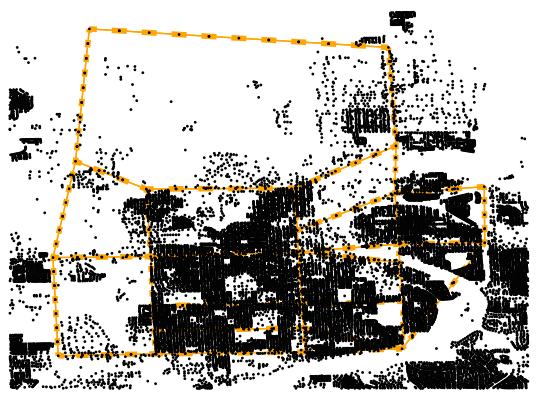
\includegraphics[width=0.80\textwidth]{img/sioux/facilities}
\caption{Rozkład budynków na grafie miasta Sioux Falls.} 
\end{figure}

Prezentuję również ruch drogowy w~najbardziej intensywnych godzinach dnia, tj. godzinach szczytu. Ruch jest przedstawiony jako natężenie ruchu na każdej krawędzi (ulicy), poprzez odniesienie go do możliwości przepustowości każdego węzła. Kolor zielony oznacza małe obciążenie, żółty średnie i~czerwony - wysokie natężenie ruchu w~tym miejscu. Obrazki są obrócone o~$90^{\circ}$ w~lewo, dla zwiększenia ich czytelności i~rozmiaru.

\begin{figure}[ht]
\centering
%bottom right top left
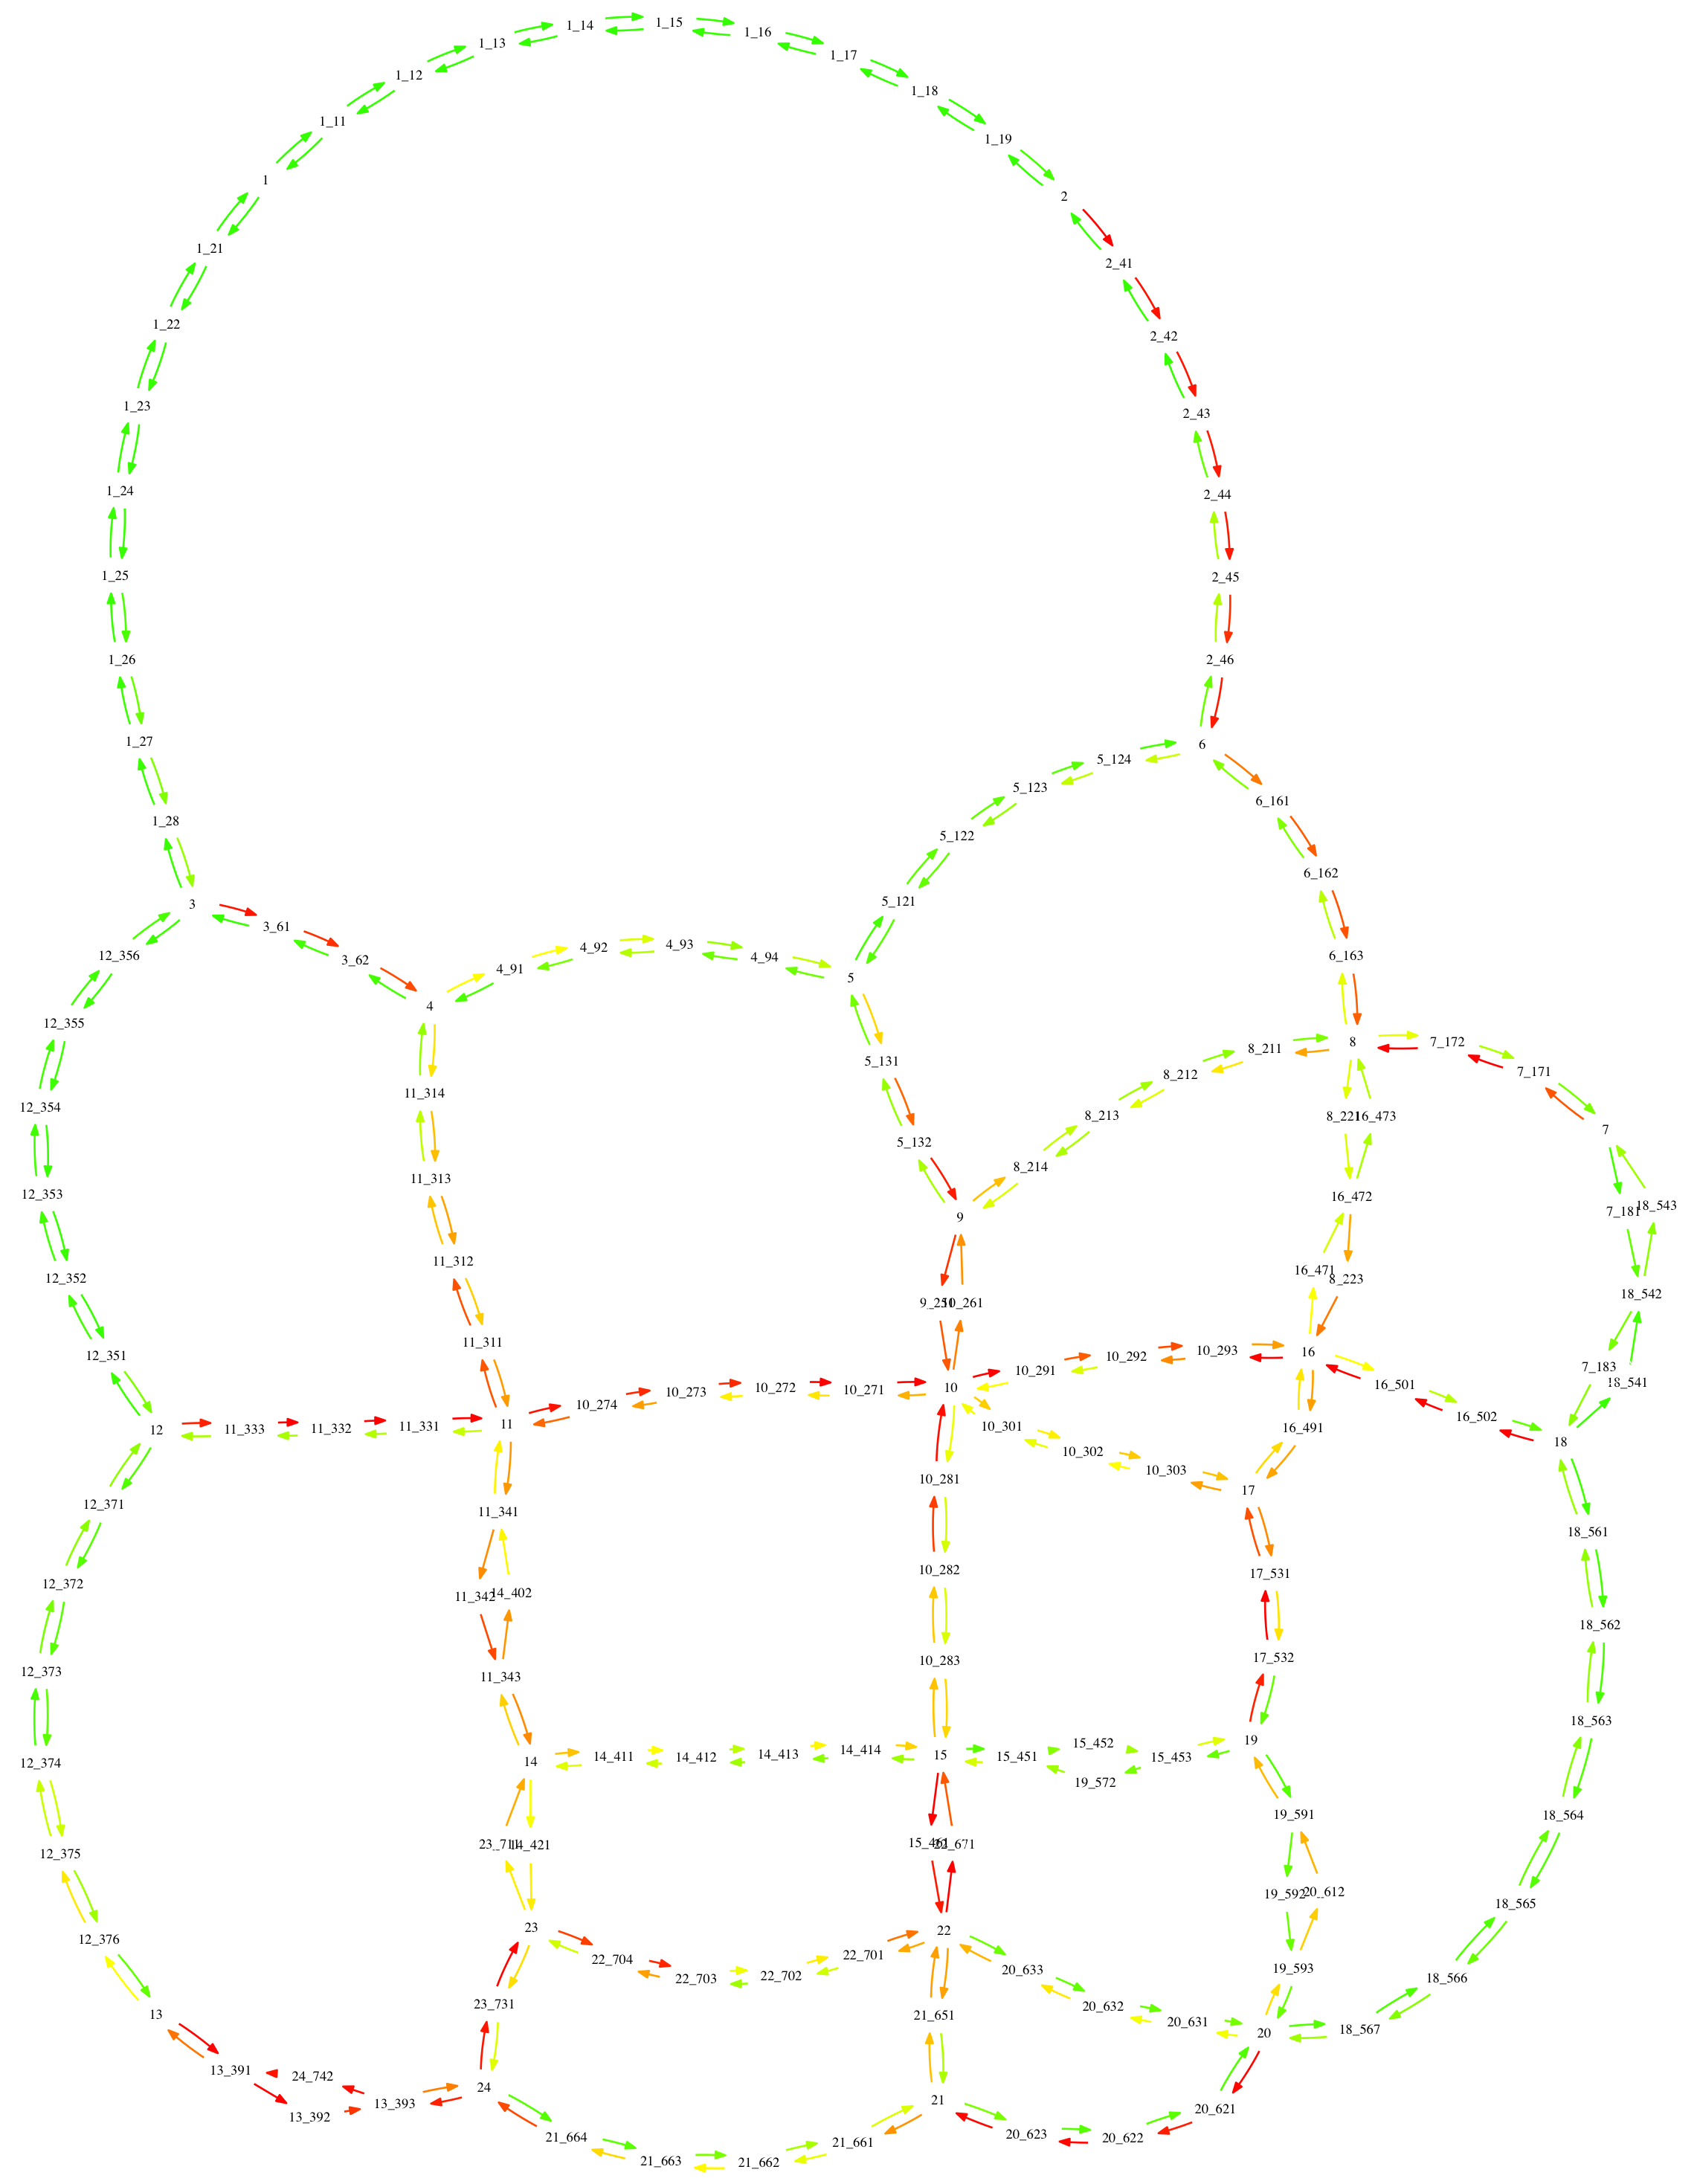
\includegraphics[trim=15cm 5cm 10cm 25cm, clip=true, totalheight=0.55\textheight, angle=90]{{{img/sioux/graph6.00-7.00}}}
\caption{Natężenie ruchu w mieście Sioux Falls w godzinach 6.00-7.00.} 
\end{figure}

\begin{figure}[ht]
\centering
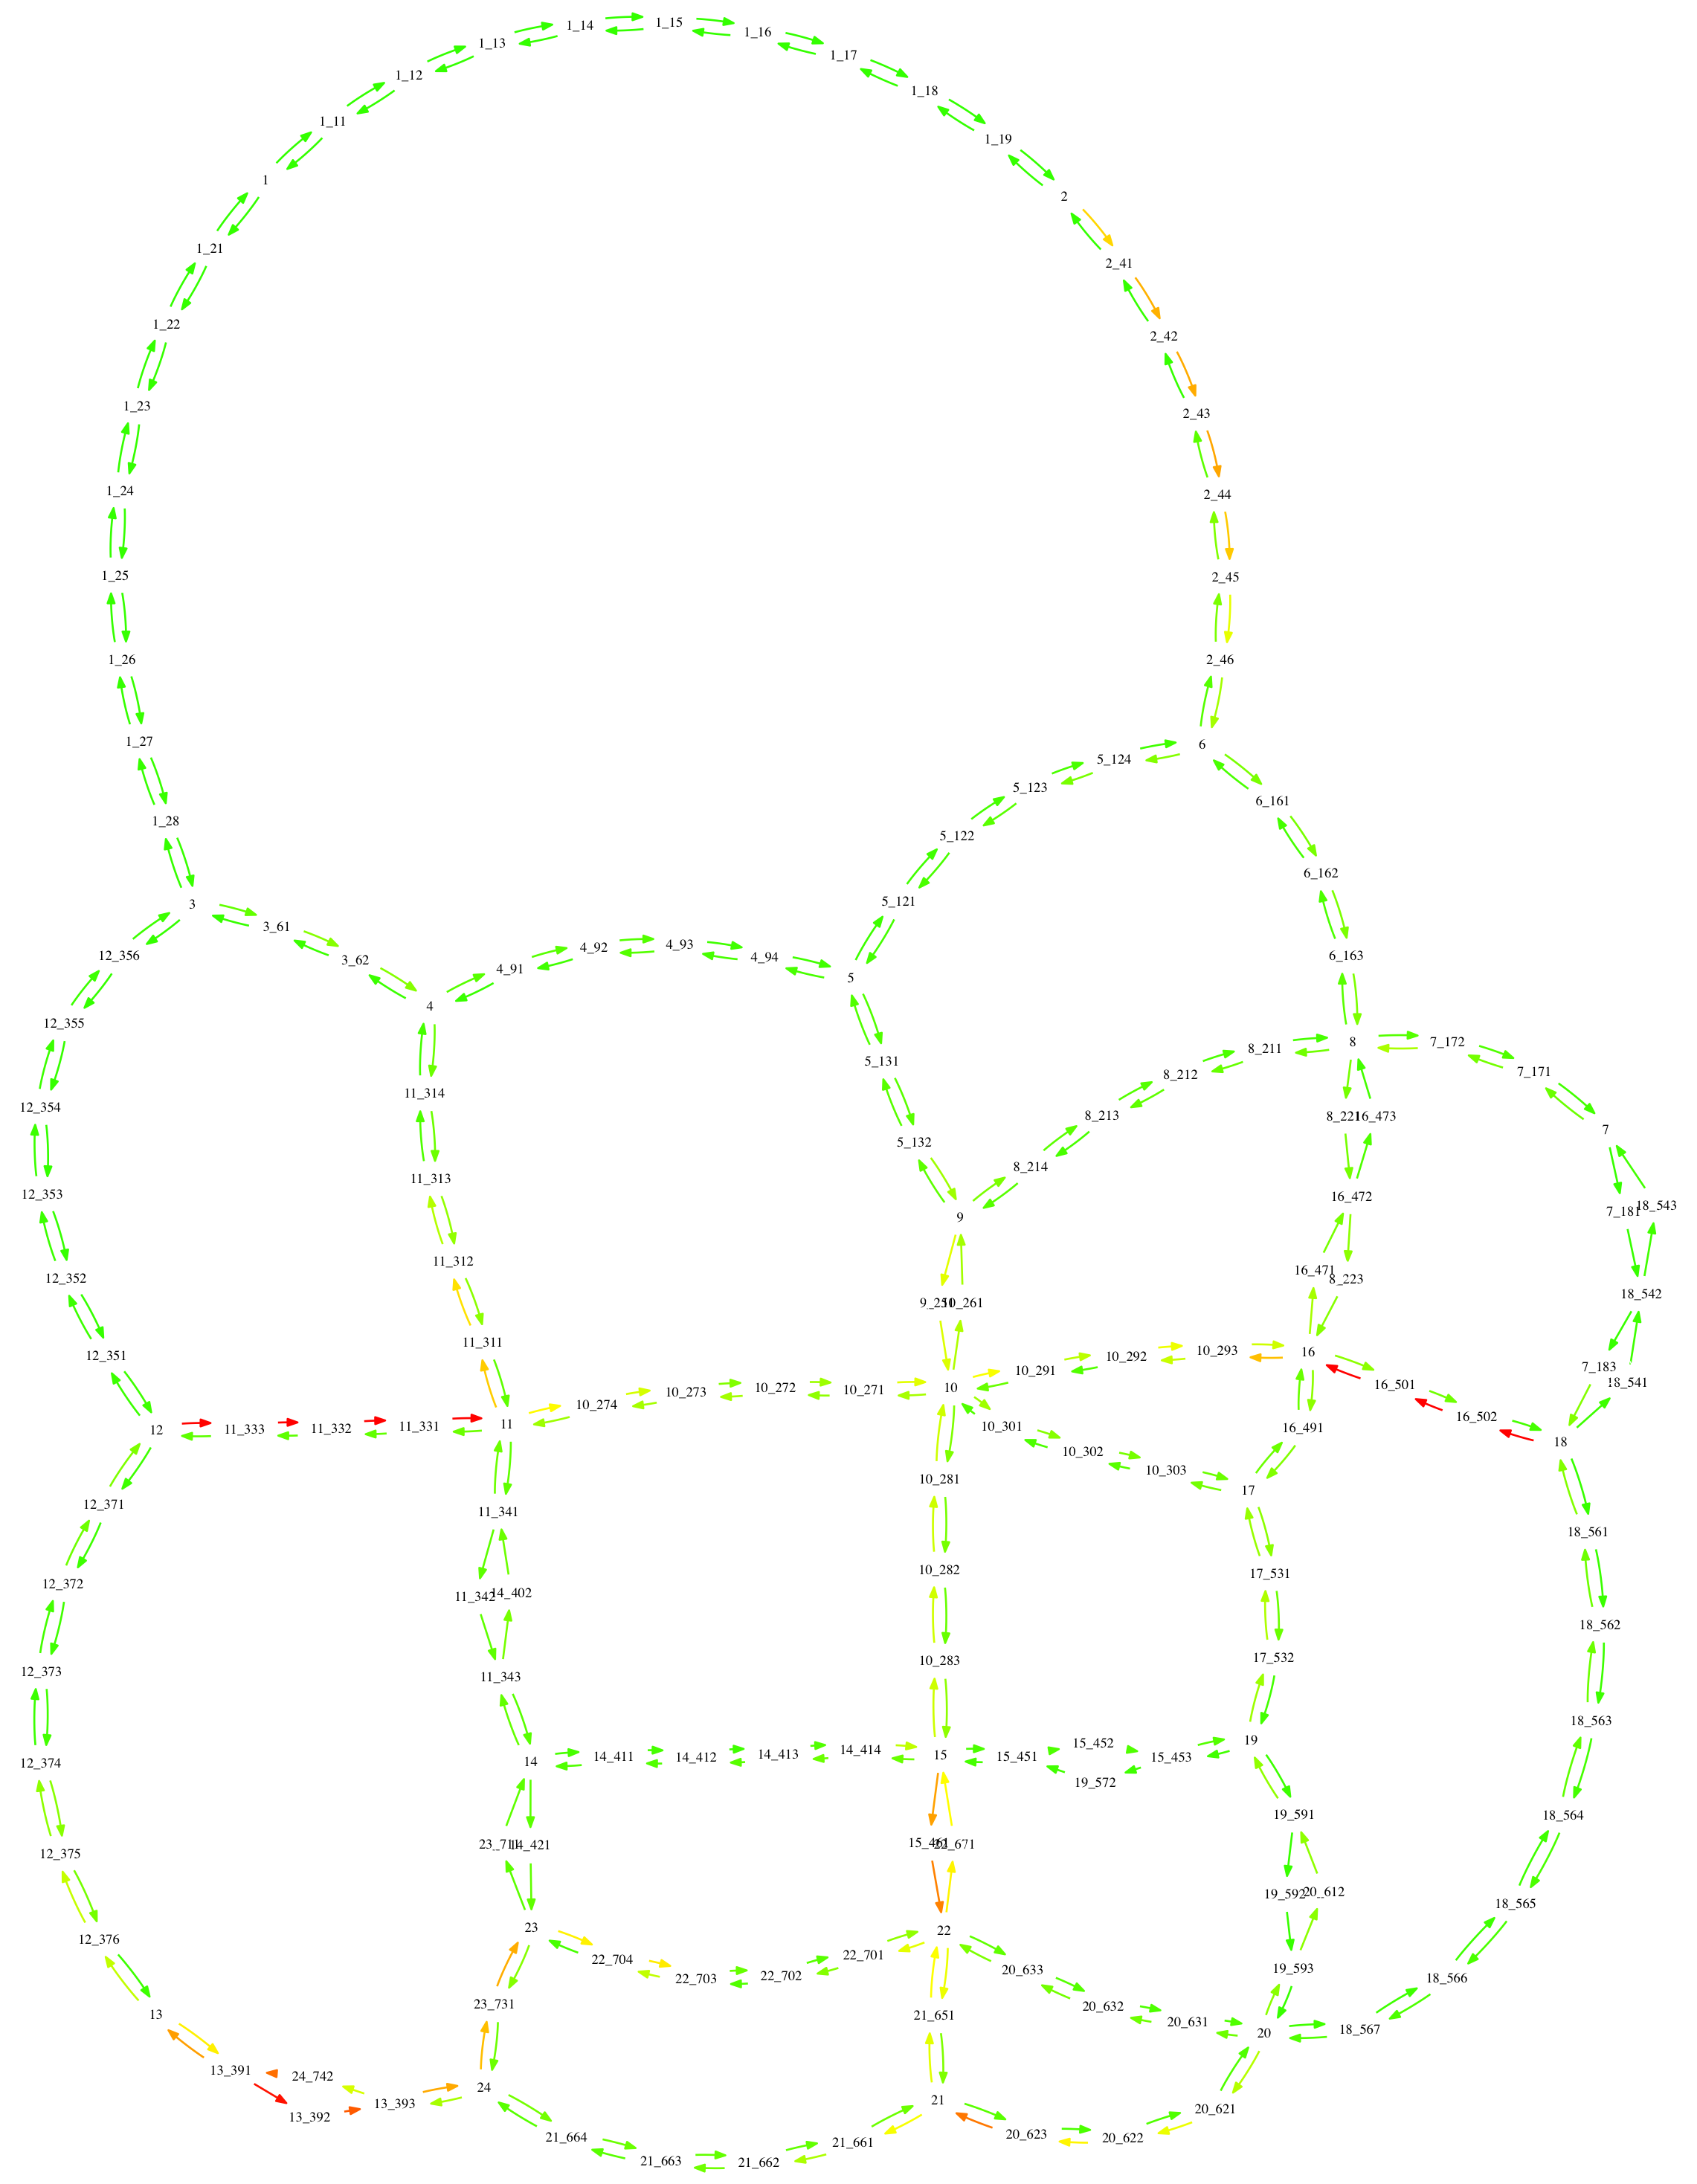
\includegraphics[trim=15cm 5cm 10cm 25cm, clip=true, totalheight=0.55\textheight, angle=90]{{{img/sioux/graph7.00-8.00}}}
\caption{Natężenie ruchu w mieście Sioux Falls w godzinach 7.00-8.00.} 
\end{figure}

\begin{figure}[ht]
\centering
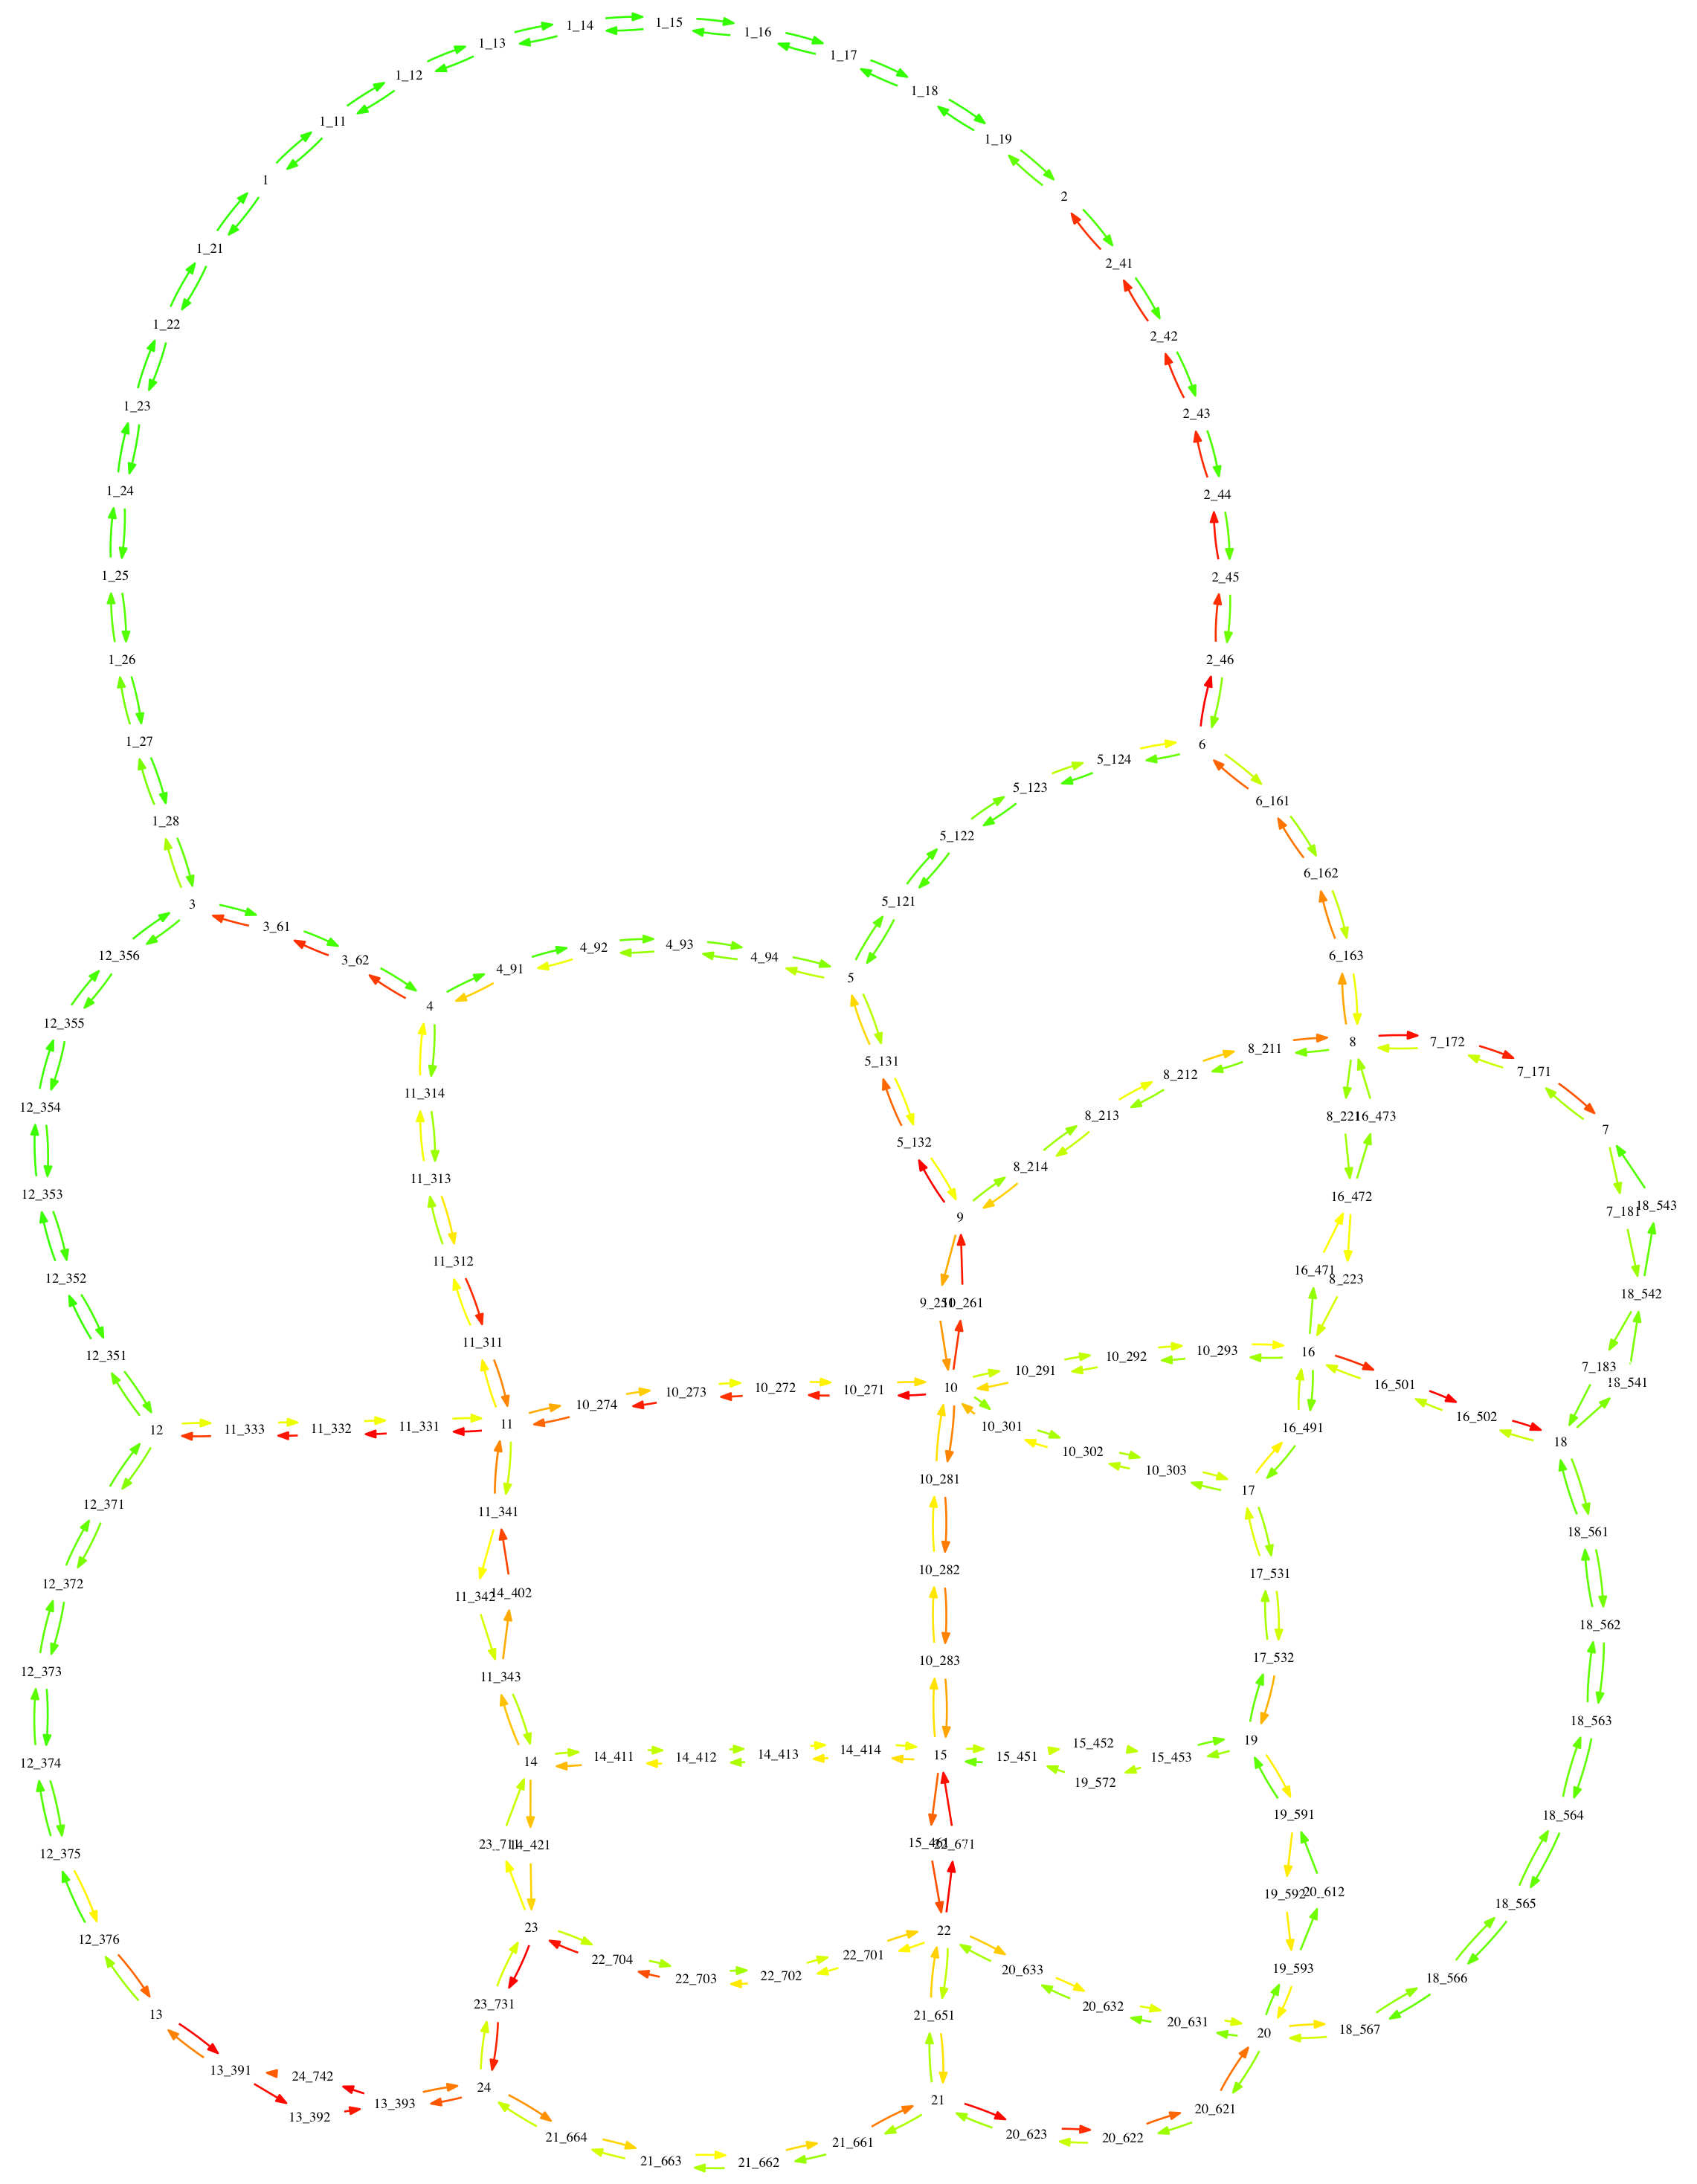
\includegraphics[trim=15cm 5cm 10cm 25cm, clip=true, totalheight=0.55\textheight, angle=90]{{{img/sioux/graph16.00-17.00}}}
\caption{Natężenie ruchu w mieście Sioux Falls w godzinach 16.00-17.00.} 
\end{figure}

\begin{figure}[ht]
\centering
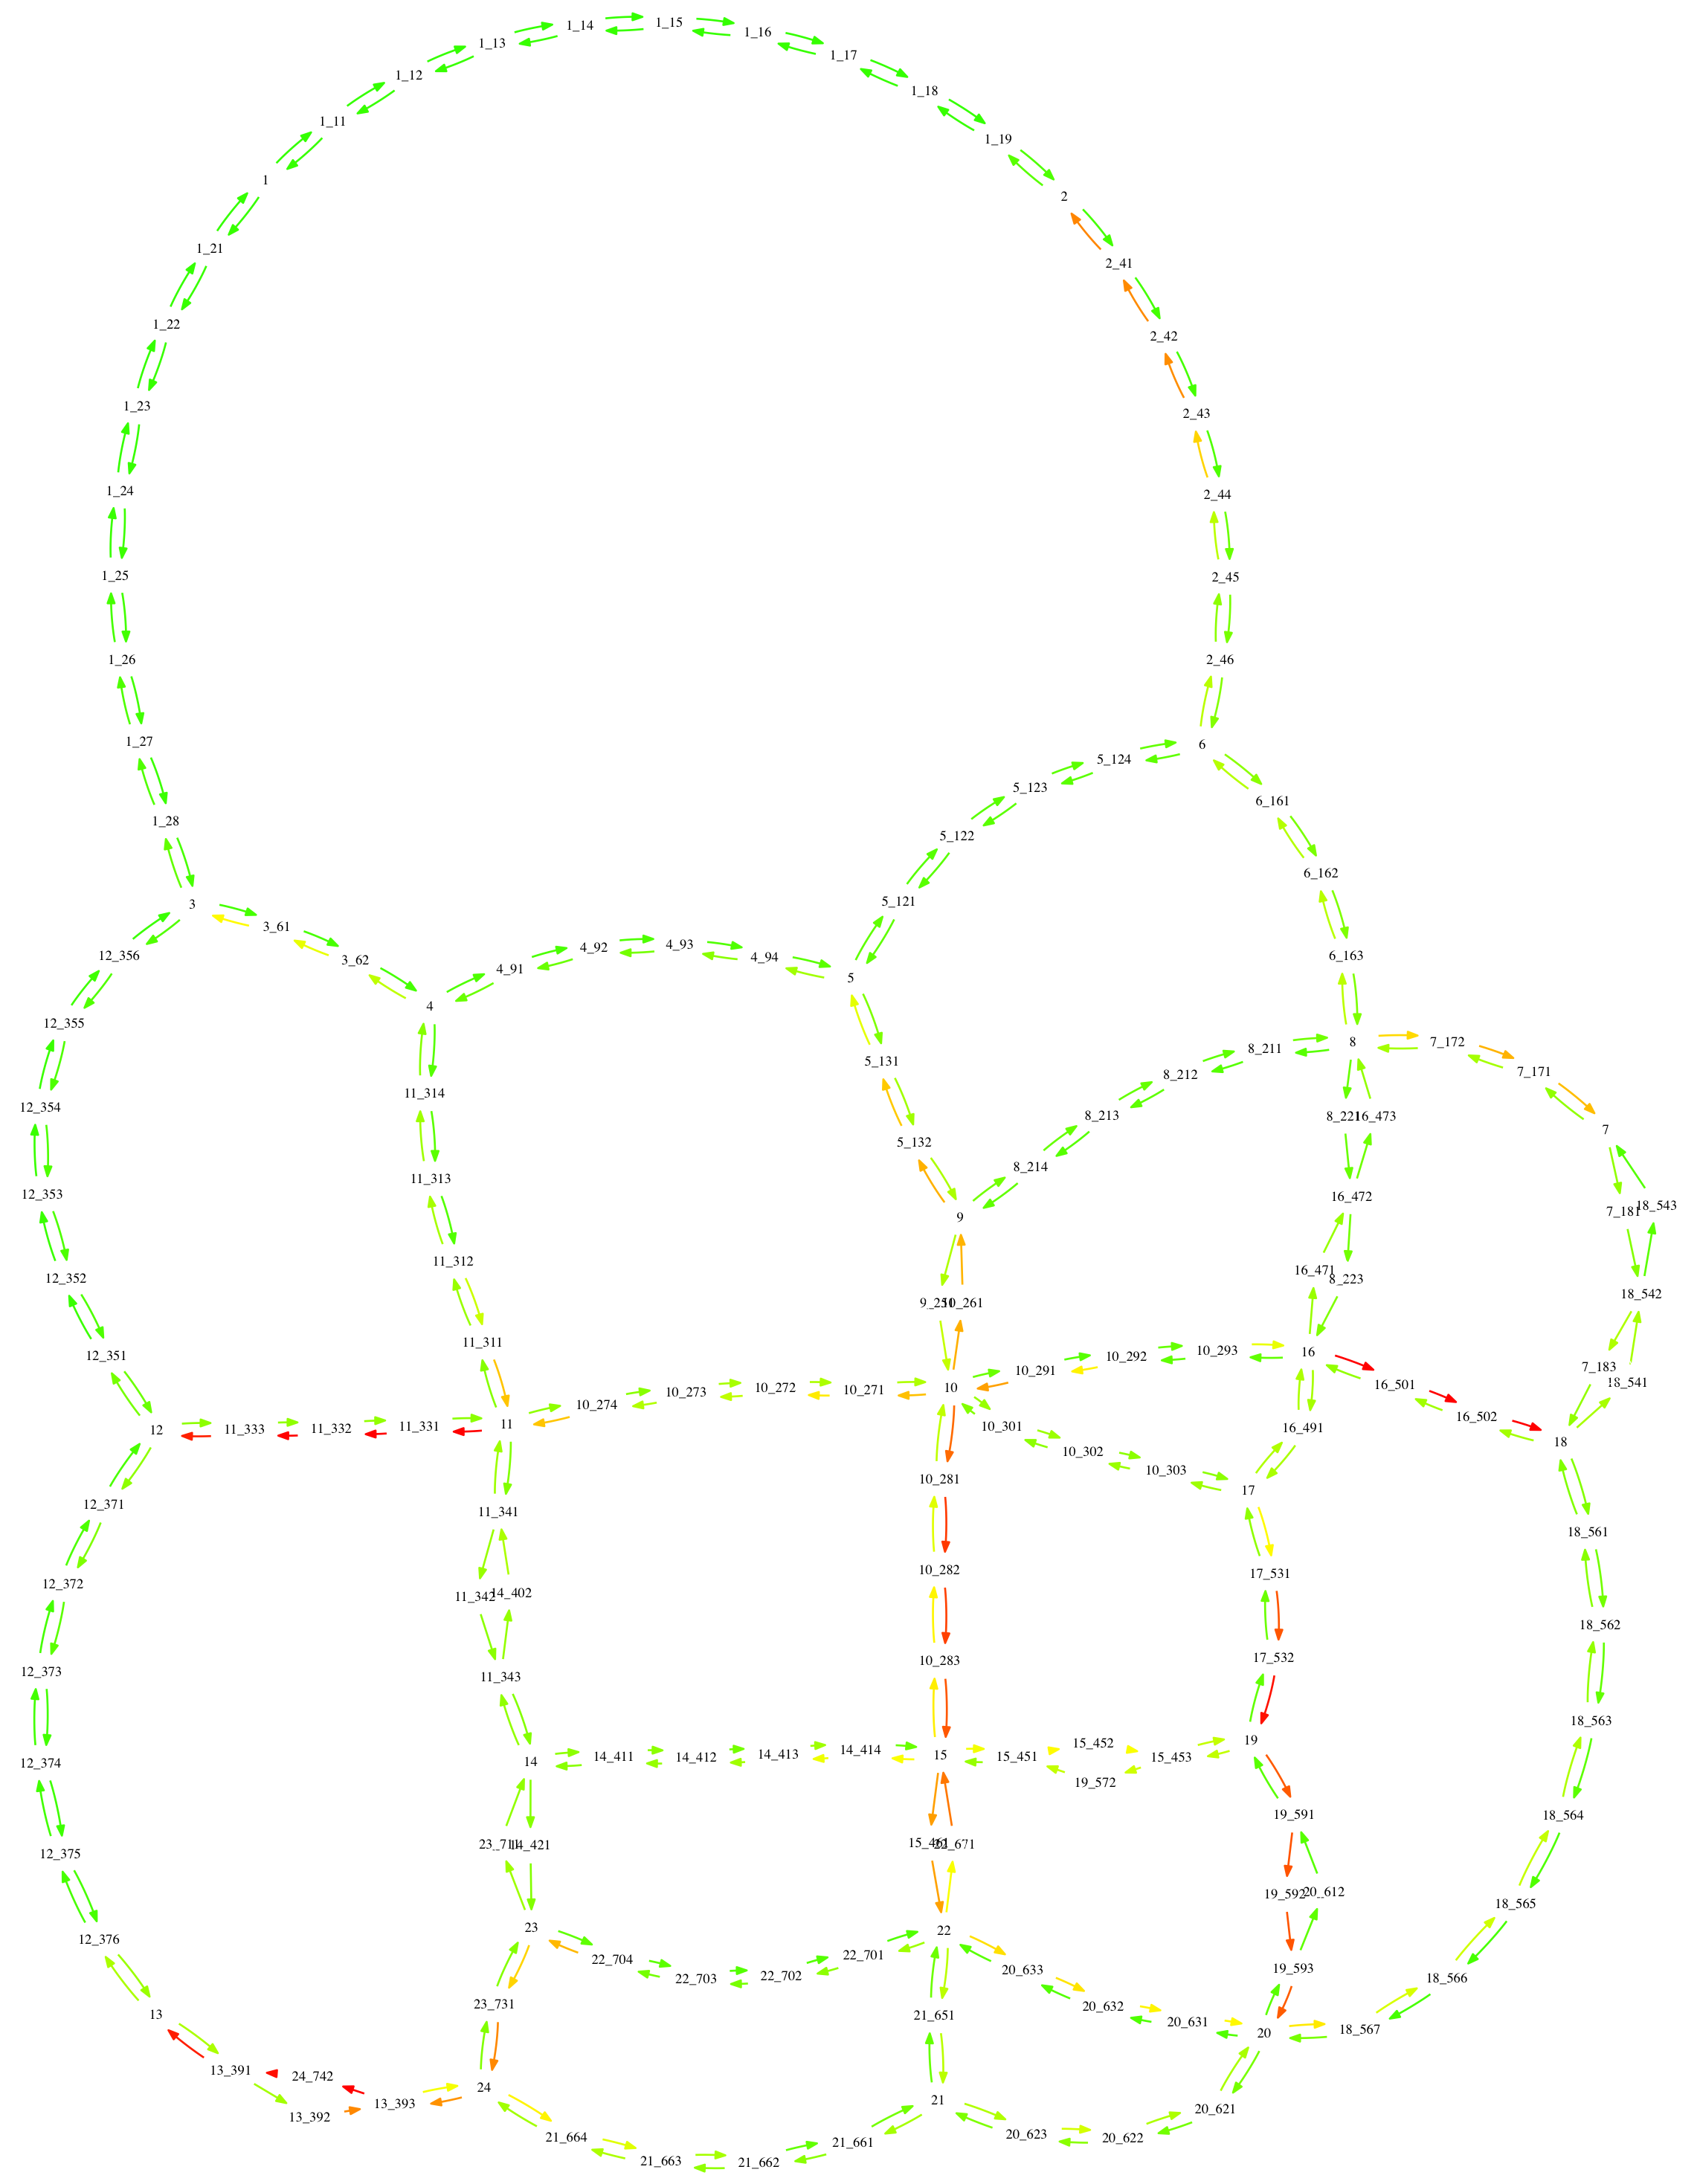
\includegraphics[trim=15cm 5cm 10cm 25cm, clip=true, totalheight=0.55\textheight, angle=90]{{{img/sioux/graph17.00-18.00}}}
\caption{Natężenie ruchu w mieście Sioux Falls w godzinach 17.00-18.00.} 
\end{figure}


\chapter{Opis projektu.}\label{rozdz.opis} 

W tym rozdziale opiszę strukturę swojego projektu z~opisem jego uruchomienia. Ponieważ przeprowadzane przez projekt obliczenia wymagają wiele czasu, zdecydowałem się na pominięcie interfejsu użytkownika przy projektowaniu aplikacji. Całość jest obsługiwana przez plik konfiguracyjny, który zostaje wczytany na początku operacji i~za jego pomocą kontrolujemy przebieg obliczeń.~Pomimo dwóch osobnych technologii, w~których wykonałem projekt, są one od siebie zależne. Całość jest obsługiwana przez projekt w~Java, skrypty w~Pythonie jedynie wspierają niektóre procesy.

\section{Dane wejściowe.}

Poniżej przedstawiam przykładowy plik konfiguracyjny dla projektu z~opisem jego funkcji.

\lstset{
    language=xml,
    tabsize=3,
    rulesepcolor=\color{gray},
    keywordstyle=\color{blue}\bf,
    stringstyle=\color{red},
    breaklines=true,
    basicstyle=\ttfamily\scriptsize}
\lstinputlisting[language=Xml, caption=Plik konfiguracyjny projektu]{img/config.xml}

\vspace*{15px}

Jak widać konfiguracja dzieli się na trzy podstawowe grupy:
\begin{itemize}
\item project,
\item scenario,
\item genetics.
\end{itemize}

\vspace*{15px}

Grupa \textit{project} odpowiada za główne ustawienia całego projektu, w~\textit{scenario} znajdziemy ustawienia dotyczące symulacji przeprowadzanej przez MATSim, natomiast sekcja \textit{genetics} zawiera ustawienia dotyczące algorytmu genetycznego.

\vspace*{15px}

Wyjaśnienie opcji \textit{project}:
\begin{itemize}
\item name - nazwa projektu, używana jako katalog wyjściowy
\item output dir - katalog, gdzie zapisujemy wyniki
\item threads - ilość wątków, które mają być użyte podczas obliczeń
\item log level - poziom logowania Log4J\footnote{zewnętrzna biblioteka do logowania, dostępne poziomy: DEBUG, INFO, WARN, ERROR i~FATAL}
\item python path - ścieżka instalacji Pythona
\item python main - folder ze skryptami pomocniczymi
\end{itemize}

\vspace*{15px}

Wyjaśnienie opcji \textit{scenario}:
\begin{itemize}
\item config - scieżka dostępu pliku konfiguracyjnego scenariusz MATSim
\item network - scieżka dostępu pliku z~siecią wejściową scenariusza
\item population - scieżka dostępu pliku z~populacja scenariusza
\item facilities - scieżka dostępu pliku z~budynkami scenariusza
\item iterations - ilość iteracji symulacji MATSima
\end{itemize}

\vspace*{15px}

Wyjaśnienie opcji \textit{genetics}:
\begin{itemize}
\item population size - rozmiar populacji
\item max generations - ilość testowanych generacji (warunek stopu)
\item elitism rate - ułamek najlepszych chromosomów populacji biorący udział w~kolejnej iteracji
\item crossover rate - szansa na krzyżowanie osobników
\item mutation rate - szansa na mutacje osobników
\item tournament rate - ilość osobników biorących udział w~turnieju
\end{itemize}


\section{Wdrożenie.}

Ze względu na duże wymagania sprzętowe obliczeń, a~zarazem ograniczoną przenośność rozwiązania z~powodu skorzystania z~Pythona, zdecydowałem się na usprawnienie rozwiązania. Wykorzystując system Linux Trisquel stworzyłem maszynę wirtualną spełniającą wszystkie wymagania do uruchomienia aplikacji. Dzięki temu mogłem wykorzystać inne maszyny oprócz tej, na której tworzyłem rozwiązanie, bez problemu przystosowania czy instalowania dużej ilości zewnętrznego oprogramowania i~bibliotek\cite{trisquel}.

\begin{figure}[ht]
\centering

\includegraphics[width=0.3\textwidth]{img/trisquel}
\caption{Logo systemu Linux Trisquel.}
\end{figure}

\section{Wyniki.}


\chapter{Podsumowanie.}\label{rozdz.podsumowanie} 
\section{Dyskusja wyników.}


\section{Perspektywy dalszych badań w~dziedzinie.}


\section{Struktura projektu.}

\cleardoublepage
\phantomsection
\addcontentsline{toc}{chapter}{\listfigurename} 
\listoffigures

\cleardoublepage
\phantomsection
\addcontentsline{toc}{chapter}{\listtablename} 
\listoftables

\cleardoublepage
\phantomsection
\addcontentsline{toc}{chapter}{\lstlistlistingname}
\lstlistoflistings

\cleardoublepage
\phantomsection
\addcontentsline{toc}{chapter}{\bibname} 
\begin{thebibliography}{99}
\bibitem{investigation} 
	Leslie Arthur Keith Bloy, 
	\newblock \textit{An investigation into Braess’ paradox}, 02/2007

\bibitem{newinsights}
	Rric Pas and Shari Principio
	\newblock \textit{Braess’ paradox: Some new insights}, April 1996

\bibitem{conference} 
	Wataru Nanya, Hiroshi Kitada, Azusa Hara, Yukiko Wakita, Tatsuhiro Tamaki, and Eisuke Kita
	\newblock \textit{Road Network Optimization for Increasing Traffic Flow}
	\newblock Int. Conference on Simulation Technology, JSST 2013.

\bibitem{reducingtheeffects}
	Ana L.~C.~Bazzan and Franziska Klügl
	\newblock \textit{Reducing the Effects of the Braess Paradox with Information Manipulation}

\bibitem{paradox}
	Dietrich Braess. 
	\newblock \textit{Über ein Paradoxon aus der Verkehrsplanung. „Unternehmensforschung”.} 
	\newblock 12, s.~258–268, 1968 (niem.).

\bibitem{gene}
	Mitchell Melanie
	\newblock \textit{An Introduction to Genetic Algorithms}
	\newblock First MIT Press paperback edition, 1998

\bibitem{matsim userg}
	M.~Rieser, C.~Dobler, T.~Dubernet, D.~Grether, A.~Horni, G.~Lammel, R.~Waraich, M.~Zilske, Kay W.~Axhausen, Kai Nagel
	\newblock \textit{MATSim User Guide}
	\newblock updated September 12, 2014

\bibitem{siux}
	A.~Chakirov
	\newblock \textit{Enriched Sioux Falls Scenario with Dynamic Demand}
	\newblock MATSim User Meeting, Zurich/Singapore, June 2013.
	
\bibitem{grafy}
	Łukasz Kowalik
	\newblock \textit{Algorytmy i~struktury danych, grafy}
	\newblock Wykład, 2003.
	
\bibitem{genetyczne}
	Marta Grzanek
	\newblock \textit{Sztuczna inteligencja, Klasyczny algorytm genetyczny}
	\newblock Wykład, 2007.
	
\bibitem{gene mutikrzyz}
	Dilvan de Abreu Moreira
	\newblock \textit{Agents: A~Distributed Client/Server System for Leaf Cell Generation}
	\newblock Thesis, 1995
	
\bibitem{matsim} 
	\url{http://matsim.org}	

\bibitem{math}
	\url{http://commons.apache.org/proper/commons math}
	
\bibitem{networkx}
	\url{http://networkx.github.io}

\bibitem{java} 
	\url{http://www.java.com/pl/}

\bibitem{eclipse} 
	\url{https://eclipse.org}
				
\bibitem{python} 
	\url{http://pl.python.org}
	
\bibitem{pydev} 
	\url{http://pydev.org}
	
\bibitem{trisquel}
	\url{https://trisquel.info}
			
\bibitem{braess}
	\url{http://pl.wikipedia.org/wiki/Paradoks_Braessa}
	
\bibitem{urban}
	\url{http://urbnews.pl/paradoks braessa/}
	
\bibitem{downs}
	\url{http://pl.wikipedia.org/wiki/Paradoks_Downsa Thomsona}
	
\bibitem{lewis}
	\href{http://pl.wikipedia.org/wiki/Prawo_Lewisa Mogridge\%E2\%80\%99a}
	    {http://pl.wikipedia.org/wiki/Prawo\_Lewisa Mogridge\textquoteright{}a}
	   
\bibitem{silniespojny}
	\url{http://mathworld.wolfram.com/StronglyConnectedDigraph.html}

\end{thebibliography}

\cleardoublepage
\phantomsection
\addcontentsline{toc}{chapter}{Abstract}
\chapter*{Abstract}


Yet to come\ldots{}



\end{document}
